\section{Patient level analysis}
\label{cascade-sec:patientLevel}
This section outlines the work performed for each patient and highlight work specifically done for certain patients due to their unique clinical features. However most of the analysis is streamlined and the workflow applied the same way to each patient. The following sections expand on the individual steps.
\begin{enumerate}
\item \textbf{Quality control:} Each sample of a patient is checked for kinship and sequencing quality
\item \textbf{Read mapping}
\item \textbf{Joint somatic variant calling:} SNPs, InDels and SVs are called jointly
\item \textbf{Copy number calling}
\item \textbf{Variant effect annotation:} short and structural variants are annotated with possible biological effects
\item \textbf{Phylogenetic reconstruction}
\item \textbf{Clonal deconvolution}
\end{enumerate}

%%%%%%%%%%%%%%%%%%%%%%%%%%%%%%%%%%%%%%%%%%%%%%%%%%%%%%%%%%%%%%%%%%%%%%%%%%%%%%%%%%%%%%%
%                               Analysis                                              %
%%%%%%%%%%%%%%%%%%%%%%%%%%%%%%%%%%%%%%%%%%%%%%%%%%%%%%%%%%%%%%%%%%%%%%%%%%%%%%%%%%%%%%%

\subsection{Analysis workflow}
\label{cascade-sec:workflow}
This section summarises the primary analysis performed for each patient in detail. Specific analysis, like RNA analysis are discussed in the individual patient sections. 

\subsubsection{Quality control}
\label{cascade-sec:qc}
When multiple samples per patient are available, the possibility of sample mix-ups and issues is higher than when just dealing with a tumour normal pair, so in addition to the standard read depth, sequencing quality and reads-on-target analysis that is routinely performed after sequencing, we performed an additional step of kinship detection. We use concepts commonly employed in germline cohort analysis, like child and parents (trio) or even large databases (gnomAD). As most germline variants are due to mendelian inheritance, we can use the percentage of shared homo- and heterozygous germline variants to estimate the relatedness of two samples. For our analysis we used NGSCheckMate \cite{Lee2017} and all the results shown in later sections are based on it, however we also used Somalier \cite{Pedersen2020} on two patient samples with surprising kinship results but Somalier confirmed the result.

While this analysis is very useful to detect samples which do not belong to a patient, either through mislabelling or similar, it does not protect from mix-ups within a patients samples. However nothing but orthogonal validation will be able to discern these errors.

Other quality controls were performed with fastQC \cite{Andrews2010} for read integrity and \lq\emph{CollectWgsMetrics}\rq~from Picard \cite{Picard2018} for WGS samples and \lq\emph{samtools flagstat}\rq~\cite{Danecek2021} for on-target estimation for WES samples.

\subsubsection{Read mapping}
\label{cascade-sec:mapping}
For highest mapping performance, reads were aligned alternative contig aware with BWA~\cite{Li2013} (v0.7.17)  to GRCh38 (\emph{GCA\_000001405.15}) with alternative contigs but no decoy regions. Initial mapping was post-processed with \lq\emph{bwa-postalt.js}\rq~from bwa-kit to adjust the mapping assignment and quality mapping both to alternative and canonical contigs. Finally reads were duplicate marked with \lq\emph{MarkDuplicates}\rq~from the Picard-toolkit.

\subsubsection{Joint somatic variant calling}
\label{cascade-sec:jsvc}
For short variants (SNPs and InDels), the workflows presented in \autoref{ch:variantcalling} were used and while the Strelka2Pass workflow generates structural variants calls, they are not jointly called over all samples. Instead for the structural variants (SVs) we used GRIDSS2 \cite{Cameron2021}, which has a calling model for multiple related tumour samples and as GRIDSS2 is also a prerequisite for copy number calling with PURPLE (\autoref{cascade-sec:cnv}) using the same structural variants allows a higher conformity of analysis.


\subsubsection{Copy number analysis}
\label{cascade-sec:cnv}
After somatic variant calling, copy number analysis is a stable when dissecting the resistance and driver alterations of a tumour sample. While lung cancers are known for their high mutational burden \cite{Alexandrov2020}, often genetic amplifications can be found as driver or resistance mechanism. One of the more common resistance mechanisms is a high \textit{EGFR} or \textit{MET} amplification which significantly affect transcription \cite{Bjaanaes2021}. And while copy number alterations are often shared between metastases \cite{Ni2013}, the same heterogeneity that can be found in variant calling analysis also affects copy number analysis. Many modern copy number calling method will use the B-allele frequency , the allele frequency of a heterozygous germline variant, to gain allele specific copy number calls \cite{Favero2015,Talevich2016,Cameron2019a}. However each of those methods will only use the input of one tumour and one germline sample, very similar to \autoref{ch:variantcalling} we can actually improve the performance by analysing all tumour samples jointly. So far only HATCHet \cite{Zaccaria2020} has a joint copy number calling method, requires significant time investment for installation and subjective manual parameter optimisation on a per patient basis. In contrast both sequenza and PURPLE have very easy installation and usage procedures.

\todo[inline]{Explain why we didnt use hatchet in the end? subjective parameter tuning?}
\todo[inline]{Explain purple vs sequenza for WGS vs WES}

\subsubsection{Variant effect annotation}
\label{cascade-sec:vep}
For small variants (SNPs and InDels) ``Variant Effect Predictor`` (VEP) version 92 \cite{McLaren2016} was used to assign possible effects. As a variant can affect multiple genes due to overlapping gene boundaries, effects within a curated list of lung cancer related genes (\autoref{A:cas:tab:lungcancergenes}) were assign an \lq\emph{IMPACT}\rq~ of \lq\emph{HIGHEST}\rq~ in order with the VEP provided impact values of \lq\emph{LOW}\rq, \lq\emph{MODERATE}\rq~ and \lq\emph{HIGH}\rq~. To only have one effect per variant, only the variant with the highest impact was returned. In case of multiple transcripts being affected with the same impact level, the putative canonical transcript result is used.

For structural variants, the effect annotation depends on the type of the structural variants. For amplifications and deletions, the genes within the variant are compiled and returned as a list. The effect of inversions and similar structural changes are assumed to be fusion based, so the breakpoint is annotated with the gene hit by both breakpoints and a potential fusion gene is returned.

\todo[color=green,inline]{potentially add the code for the effect annotation}

\subsubsection{Phylogenetic reconstruction}
\label{cascade-sec:phylo}

\subsubsection{Clonal deconvolution}
\label{cascade-sec:clonaldecon}

Clonal deconvolution for each patient was done with PhylogicNDT. To ensure high quality reconstruction, variants were filtered if the depth of coverage is lower than 8. All other called variants were transformed into the input format required in R. Cancer cell fractions (CCF) were left to PhylogicNDT with the option \lq\emph{--maf\_input\_type calc\_ccf}\rq~ by supplying the allele specific local copy number call for each variant the same way as shown in \autoref{variantcalling-sec:clonal} with the copy number calls from \autoref{cascade-sec:cnv}.


%%%%%%%%%%%%%%%%%%%%%%%%%%%%%%%%%%%%%%%%%%%%%%%%%%%%%%%%%%%%%%%%%%%%%%%%%%%%%%%%%%%%%%%
%                               Patient CA99                                          %
%%%%%%%%%%%%%%%%%%%%%%%%%%%%%%%%%%%%%%%%%%%%%%%%%%%%%%%%%%%%%%%%%%%%%%%%%%%%%%%%%%%%%%%

\subsection{Patient CA-A}
\label{cascade-sec:CA99}

This patient was a 61 year old male  with a metastatic \textit{RET-KIF5B} fusion positive NSCLC. After failure of Carboplatin, Pemetrexed, and Pembrolizumab as well as Lenvatinib, with compassionate access to Selpercatinib (\autoref{fig:ca99timeline}) he experienced almost immediate improvement with decreased levels of carcinoembryonic antigen and almost 100\% reduction of fusion positive ctDNA after one month (\autoref{fig:ca99ctDNA}). Similar to the ctDNA analysis, Positron emission tomography-computed tomography imaging revealed significantly reduced tracer uptake in multiple sites and partial response (\autoref{fig:ca99pet}).

\begin{figure}[ht]
\centering
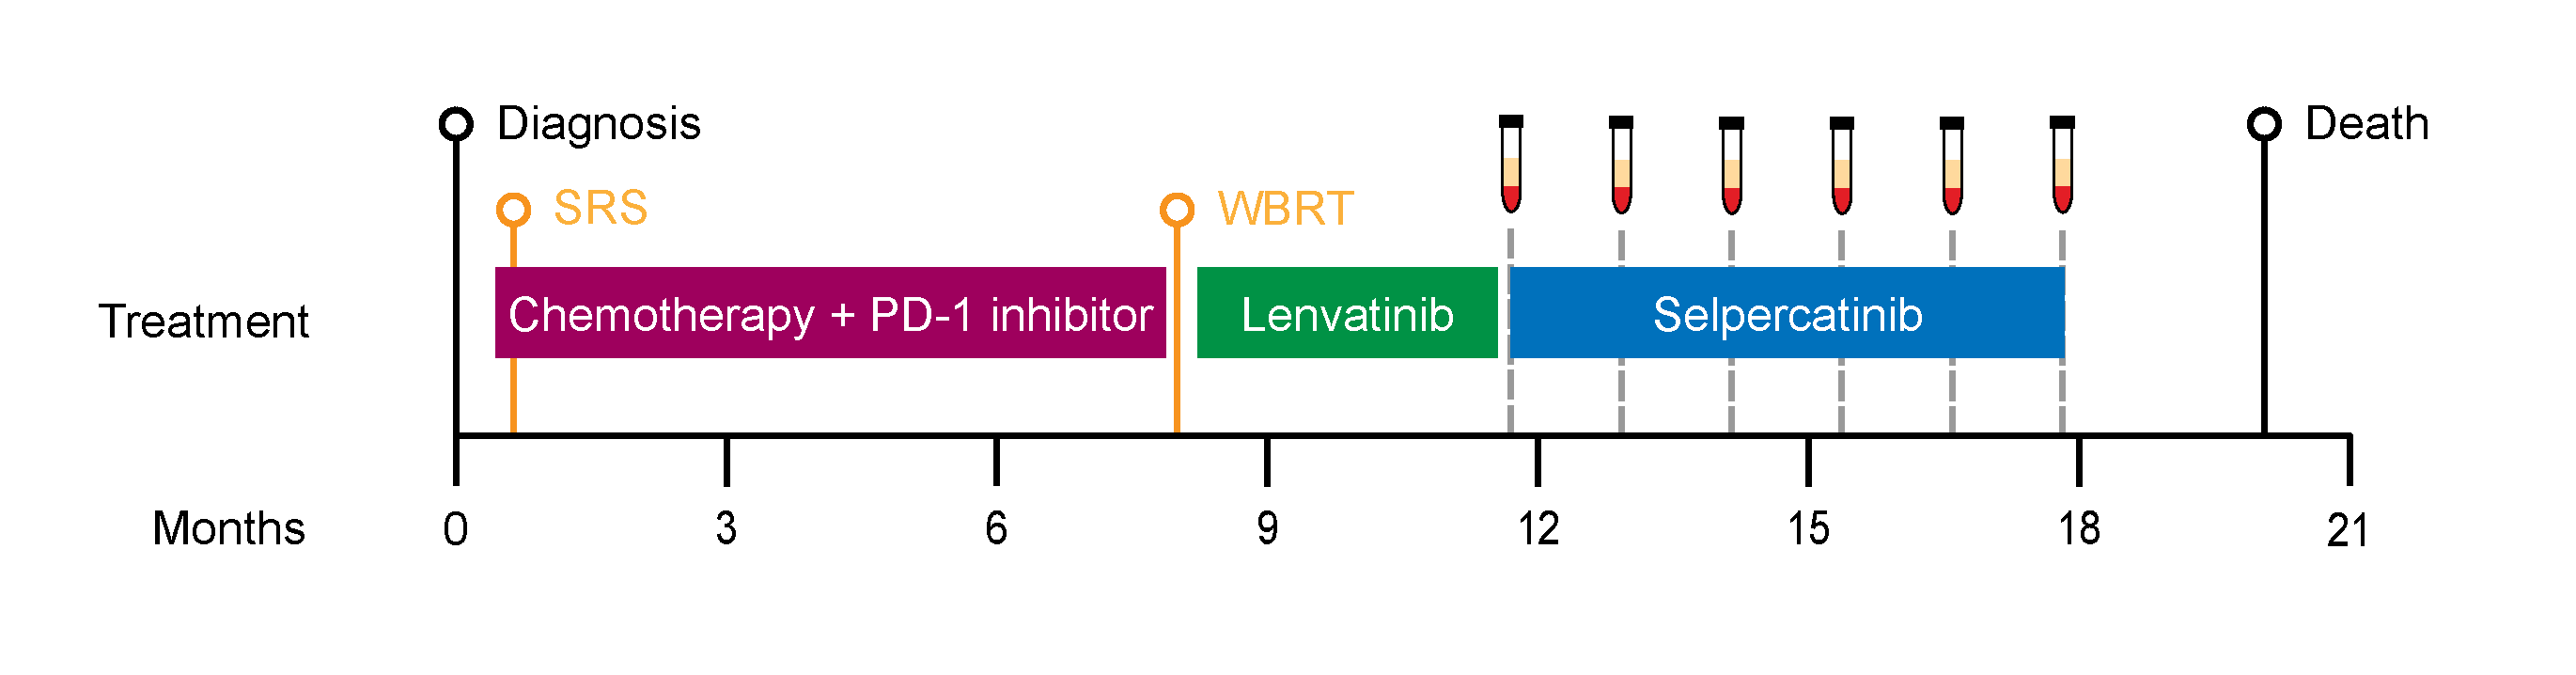
\includegraphics[width=.99\linewidth]{Figures/CASCADE/CA99/CA-A_timeline}
\caption[Timeline of patient CA-A from diagnosis until death]{Timeline of patient CA-A from diagnosis until death: Diagnostic biopsy detected \textit{KIF5B-RET} positive lung adenocarcinoma; SRS: stereotactic radiosurgery; WRBT: whole brain radiation therapy; a total of six blood samples were taken just before and during the selpercatinib treatment.} \label{fig:ca99timeline}
\end{figure}


Serial sampling of the plasma of the patient and analysis with the commercial Guardant360 assay \cite{Talasaz2014} revealed the previously undetected RET~G810S resistance mutation after three months of treatment . While at this point the driver mutation allele frequency was still dropping in the plasma, by month four the abundance of RET~G810S had increased and was accompanied by additional mutations in the same site (RET~G810R, C and V). In addition with the increase of fusion positive ctDNA this suggests that any mutation in this site affects the efficiency of Selpercatinib. While the patient initially was responsive to the treatment, repeat PET scans showed a progressive disease after six months, which ultimately lead to the death of the patient (\autoref{fig:ca99pet}).

\begin{figure}[ht]
\centering
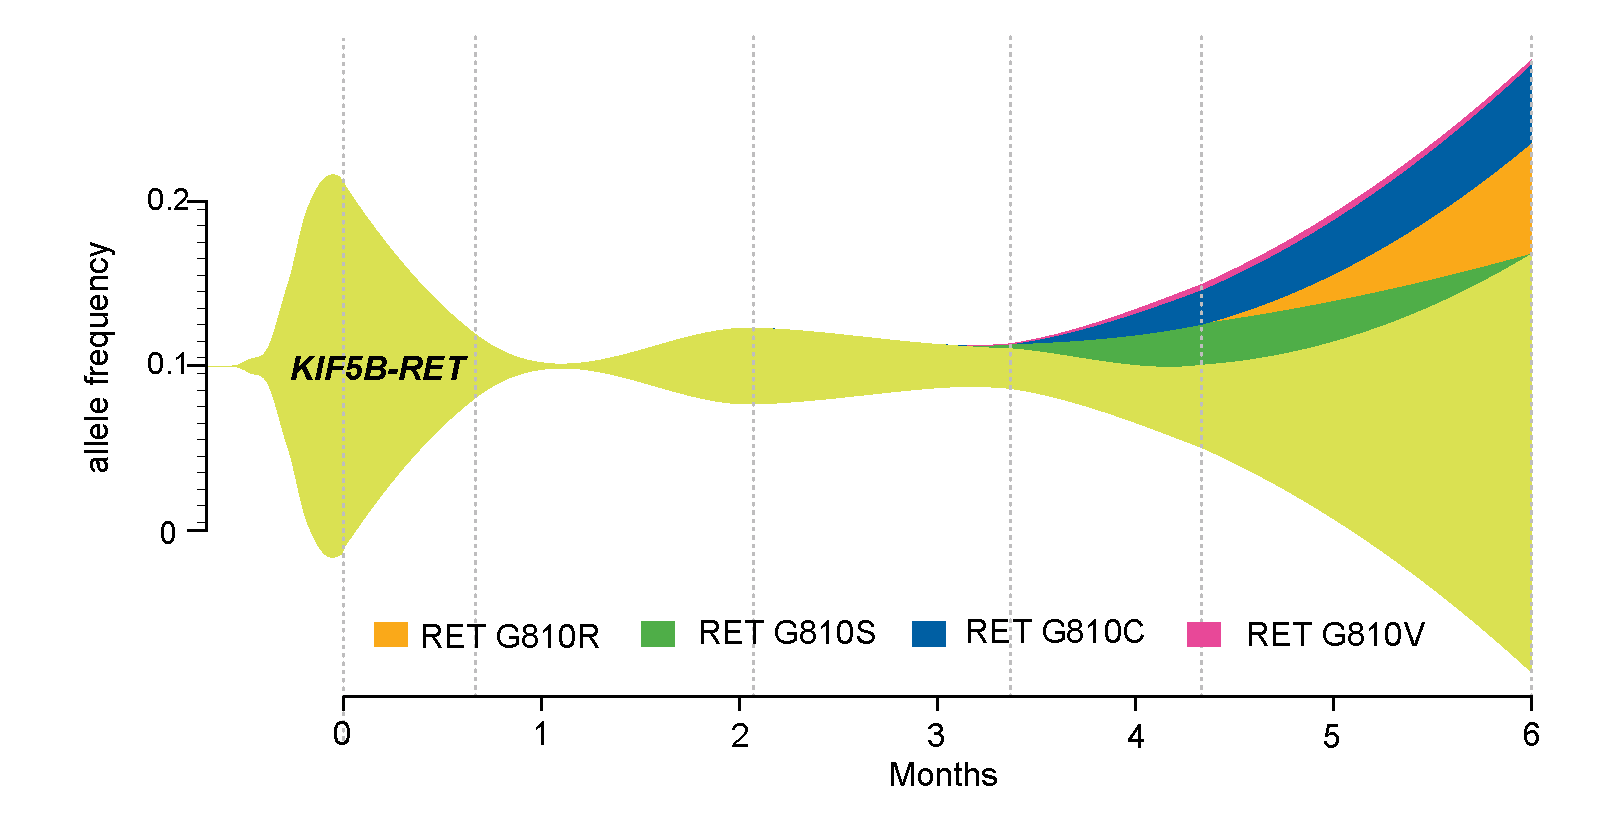
\includegraphics[width=.99\linewidth]{Figures/CASCADE/CA99/CA-A_ctDNAstream}
\caption[Allelic frequencies of of driver and emerging resistance mutations]{Allelic frequencies of of driver and emerging resistance mutations during Selpercatinib treatment (11 months after diagnosis); \textit{KIF5B-RET} fusion is the initiating driver with RET~G810R/S/C/V the emerging resistance SNPs} \label{fig:ca99ctDNA}
\end{figure}


\begin{figure}[ht]
\centering
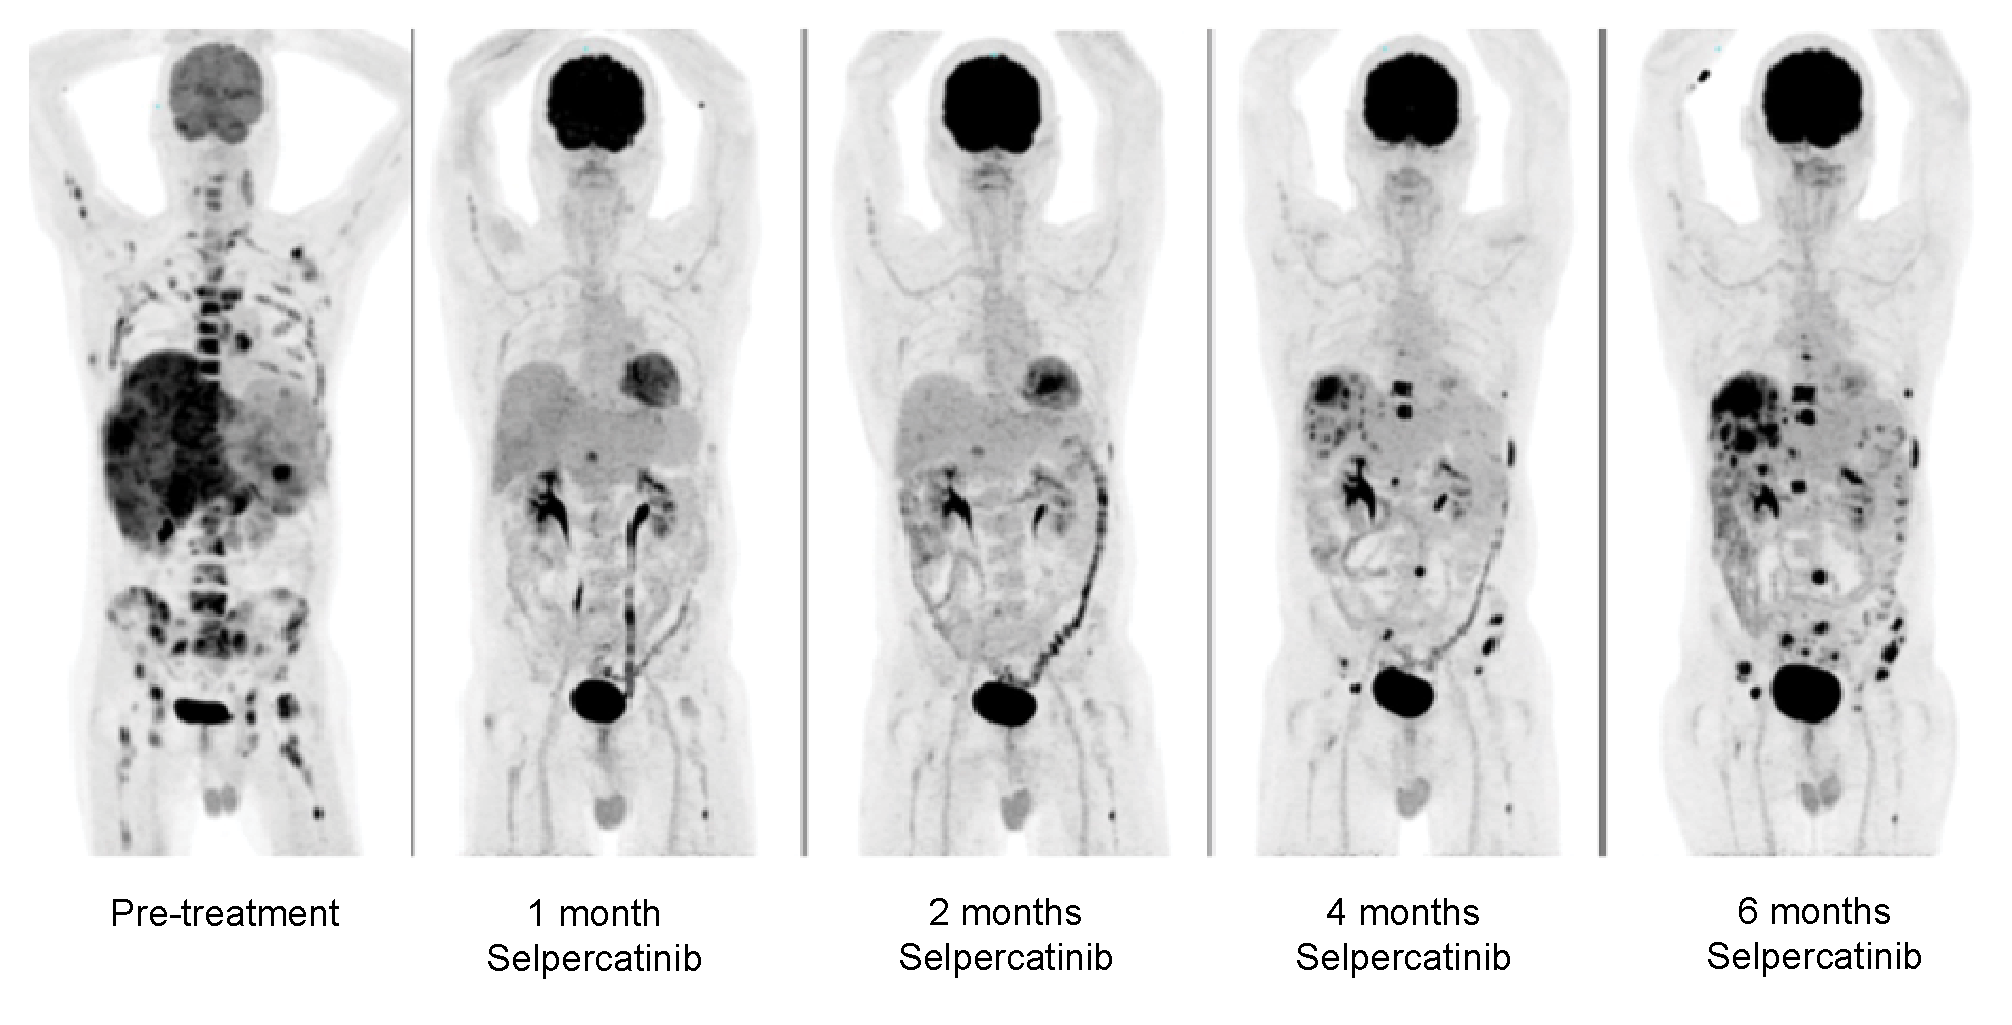
\includegraphics[width=.99\linewidth]{Figures/CASCADE/CA99/CA-A_PETscans}
\caption[PET scans of patient CA-A before and during Selpercatinib treatment]{PET scans of patient CA-A before and during Selpercatinib treatment} \label{fig:ca99pet}
\end{figure}


\begin{figure}[ht]
\centering
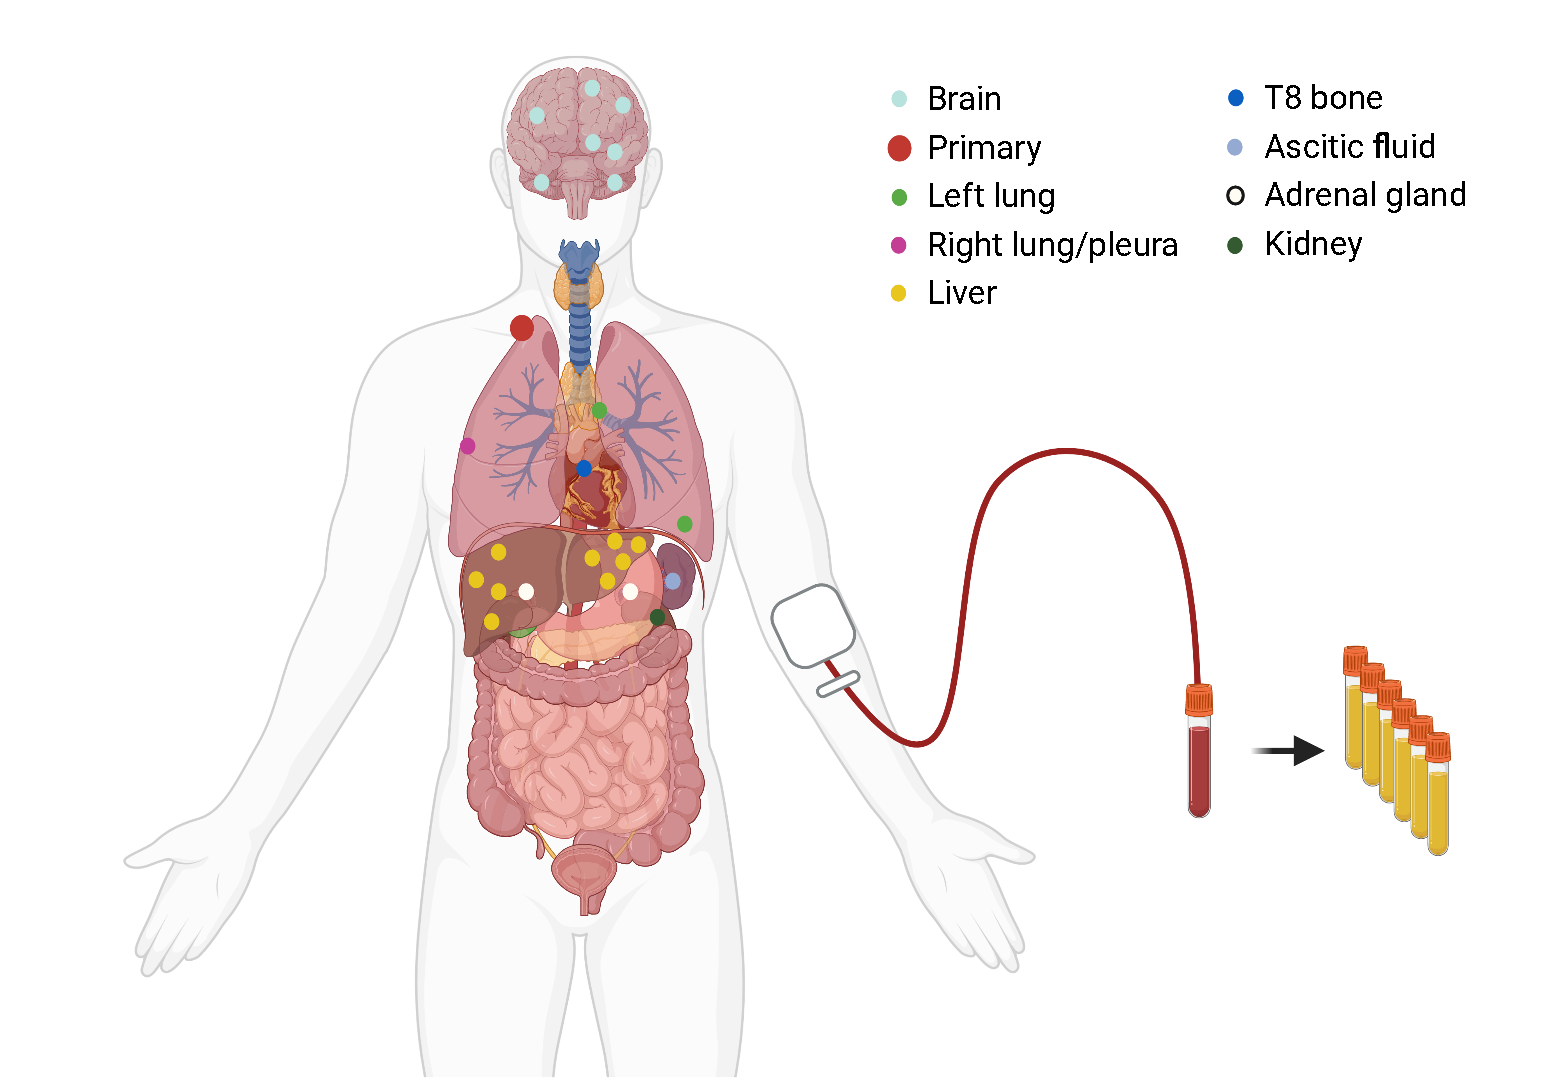
\includegraphics[width=.99\linewidth]{Figures/CASCADE/CA99/CA-A_schematic_CA99_organColours}
\caption[Schematic of tumour lesions in patient CA-A]{Schematic of tumour lesions in patient CA-A: Primary diagnostic sample shown in red; All 24 autopsy samples were coloured by organ they were collected from: Brain (7), left lung (2), right lung (1), liver (9), T8 bone (1), ascitic fluid (1), adrenal gland (2), kidney (1); Additionally to the post mortem blood sample, six serial blood samples were taken (\protect\autoref{fig:ca99timeline})} \label{fig:ca99schematic}
\end{figure}


At autopsy, 24 tumour tissue biopsies and a post mortem blood sample were collected and eight of them were selected for WGS at 130x coverage (\autoref{fig:ca99schematic}, \autoref{tab:ca99wgsSamples}\todo{add that info or remove the column}) and analysed with the standard workflow (\autoref{cascade-sec:workflow}).

\begin{table}[ht]
\caption[Autopsy samples sequenced for patient CA-A]{Autopsy samples sequenced for patient CA-A: Sample number is the internal sample collection during CASCADE autopsy, the organ of the sample, the fraction of tumour cell from H\& E stain and the pathology of the tumour sample.}\label{tab:ca99wgsSamples}
\centering
\rowcolors{2}{gray!15}{white}
\begin{tabular}{|c|c|c|c|c|}
\toprule
\hline
 \rowcolor{gray!50}
\textbf{Sample number} & \textbf{Organ} & \textbf{H \& E} & \textbf{Type}\\
\hline
 11 & right occipital lobe & 0.75 &  \cellcolor{white}\\
 26 & right liver lobe & 0.6 & \cellcolor{white} \\
 31 & left lower lung & 0.2 & \cellcolor{white} \\
 41 & left liver lobe & 0.2 & \cellcolor{white} \\
 47 & left liver lobe & 0.5 & \cellcolor{white} \\
 55 & left liver lobe & 0.4 & \cellcolor{white} \\
 57 & right liver lobe & 0.6 & \cellcolor{white} \\
 59 & right pleura & 0.7 & \cellcolor{white}\multirow{-8}{*}{lung adenocarcinoma} \\
 \hline
\bottomrule
\end{tabular}
\end{table} 

Somatic variant calling revealed substantial spatial heterogeneity, where both the occipital and the right pleura sample only contained RET~G810S, the right liver lobe harboured predominantly RET~G810R with either G810S and G810C as minor clones and lastly, the left liver samples showed almost even mix between G810C and G810S clones but no G810R presence \todo{do i need a figure here, like in the paper?}. The emergence of these mutations in multiple different sites at different allele frequencies, especially in already established sites in the liver, suggests that these mutations are the result of parallel evolution under positive selection through therapy, rather than seeding from one resistant clone.
Apart from the mutations changing RET~G810 no other variants affecting \textit{RET} or any other lung cancer genes were found in multiple samples. The occipital sample also contained a BRCA1~V939A  mutation and one left liver sample (47) showed a synonymous KIT~S967\%3D mutation. Additionally, no other variant found in non cancer related genes allowed the same explanation of resistance

The structural variant calling with GRIDSS showed consistent presence of the \textit{KIF5B-RET} fusion at high allele frequency (min: 0.27 max: 0.535), consistent with cancer cell fraction of 1 when correcting for local copy number changes  (min: 2 max: 3\todo{do i put a table or a figure here?}), in all but sample 31, which might be due to the low purity of the sample (\autoref{tab:ca99wgsSamples}). While there is a high number of structural variants present in each sample, consistent with genomic instability in late stages of cancer \cite{Gerstung2020} and wide spread chromosomal rearrangement as a hallmark of cancer \cite{Hanahan2022}, most of these rearrangements are sub-clonal and therefore not the main cause of resistance or cancer initiation and rather the result of rampant tumour evolution. To allow a more focused look at structural events and their effect, we restricted the visualisation to events with an allele frequency of 0.2 or higher (compare \autoref{fig:ca99.11circosnoAF} and \autoref{fig:ca99.11circos}).

While this change also have a minute effect on the PURPLE copy number calls, which are informed by structural variants, these structural variants will also be sub-clonal and therefore removal will result in a cleaner clonal copy number profile.

\begin{figure}[ht]
\centering
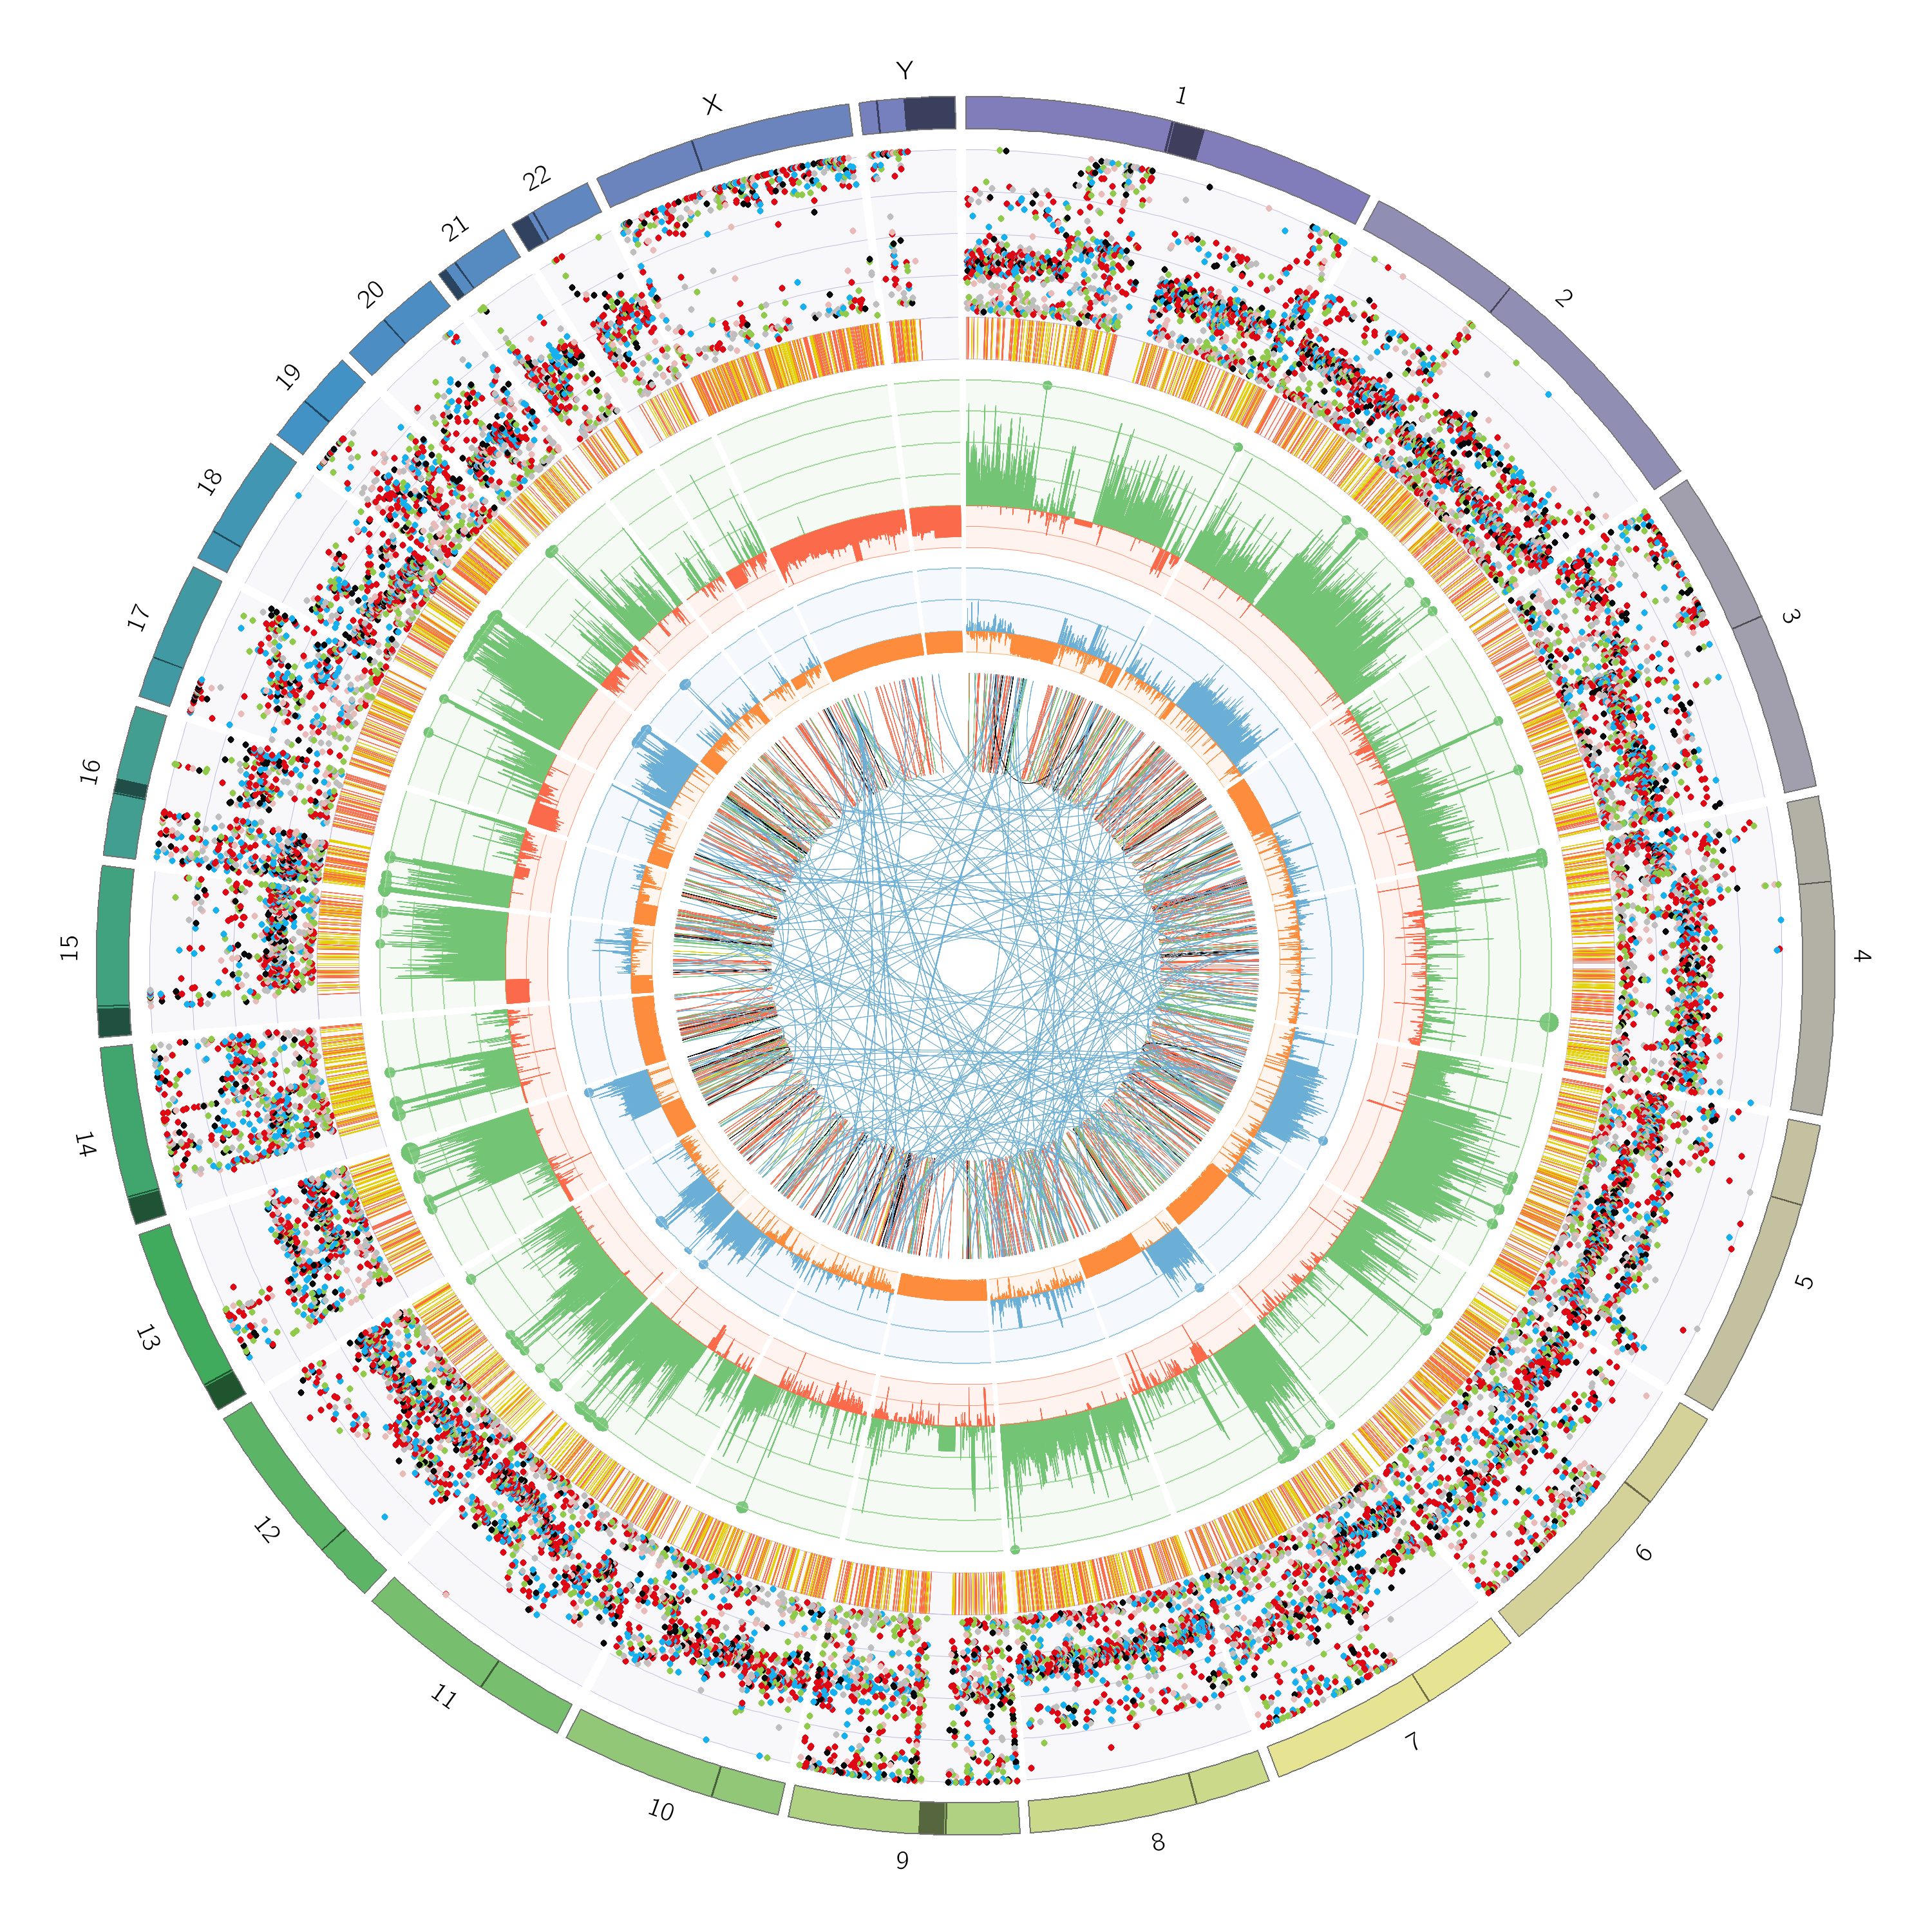
\includegraphics[width=.99\linewidth]{Figures/CASCADE/CA99/CA99-11.circos_0.05AF.png}
\caption[Circos plot of patient CA-A sample 11 without allele frequency filter]{Circos plot of patient CA-A with all somatic structural variants: outer first ring shows the canonical chromosomes with gaps (centromere, heterochromatin,...) highlighted as darker areas; second ring visualises all somatic SNVs corrected for tumour purity and scaled from 0 to 1, the colour representing the base change of SNV like in \protect\textcite{Alexandrov2013}; vertical lines directly under the SNVs symbolise InDels, with yellow for insertions and red for deletions; the third ring shows the total copy number alterations, with green showing a copy number gain and red a loss, dots at the outer border show a copy number greater than four; the last ring shows the minor copy number, with blue depicting a gain and orange a loss, this ring allows the detection of copy number neutral changes, like loss of heterozygosity; the center shows all structural variants: translocations in blue, deletions in red, insertions in yellow, tandem duplications in green and inversions in black.} \label{fig:ca99.11circosnoAF}
\end{figure}

\begin{figure}[ht]
\centering
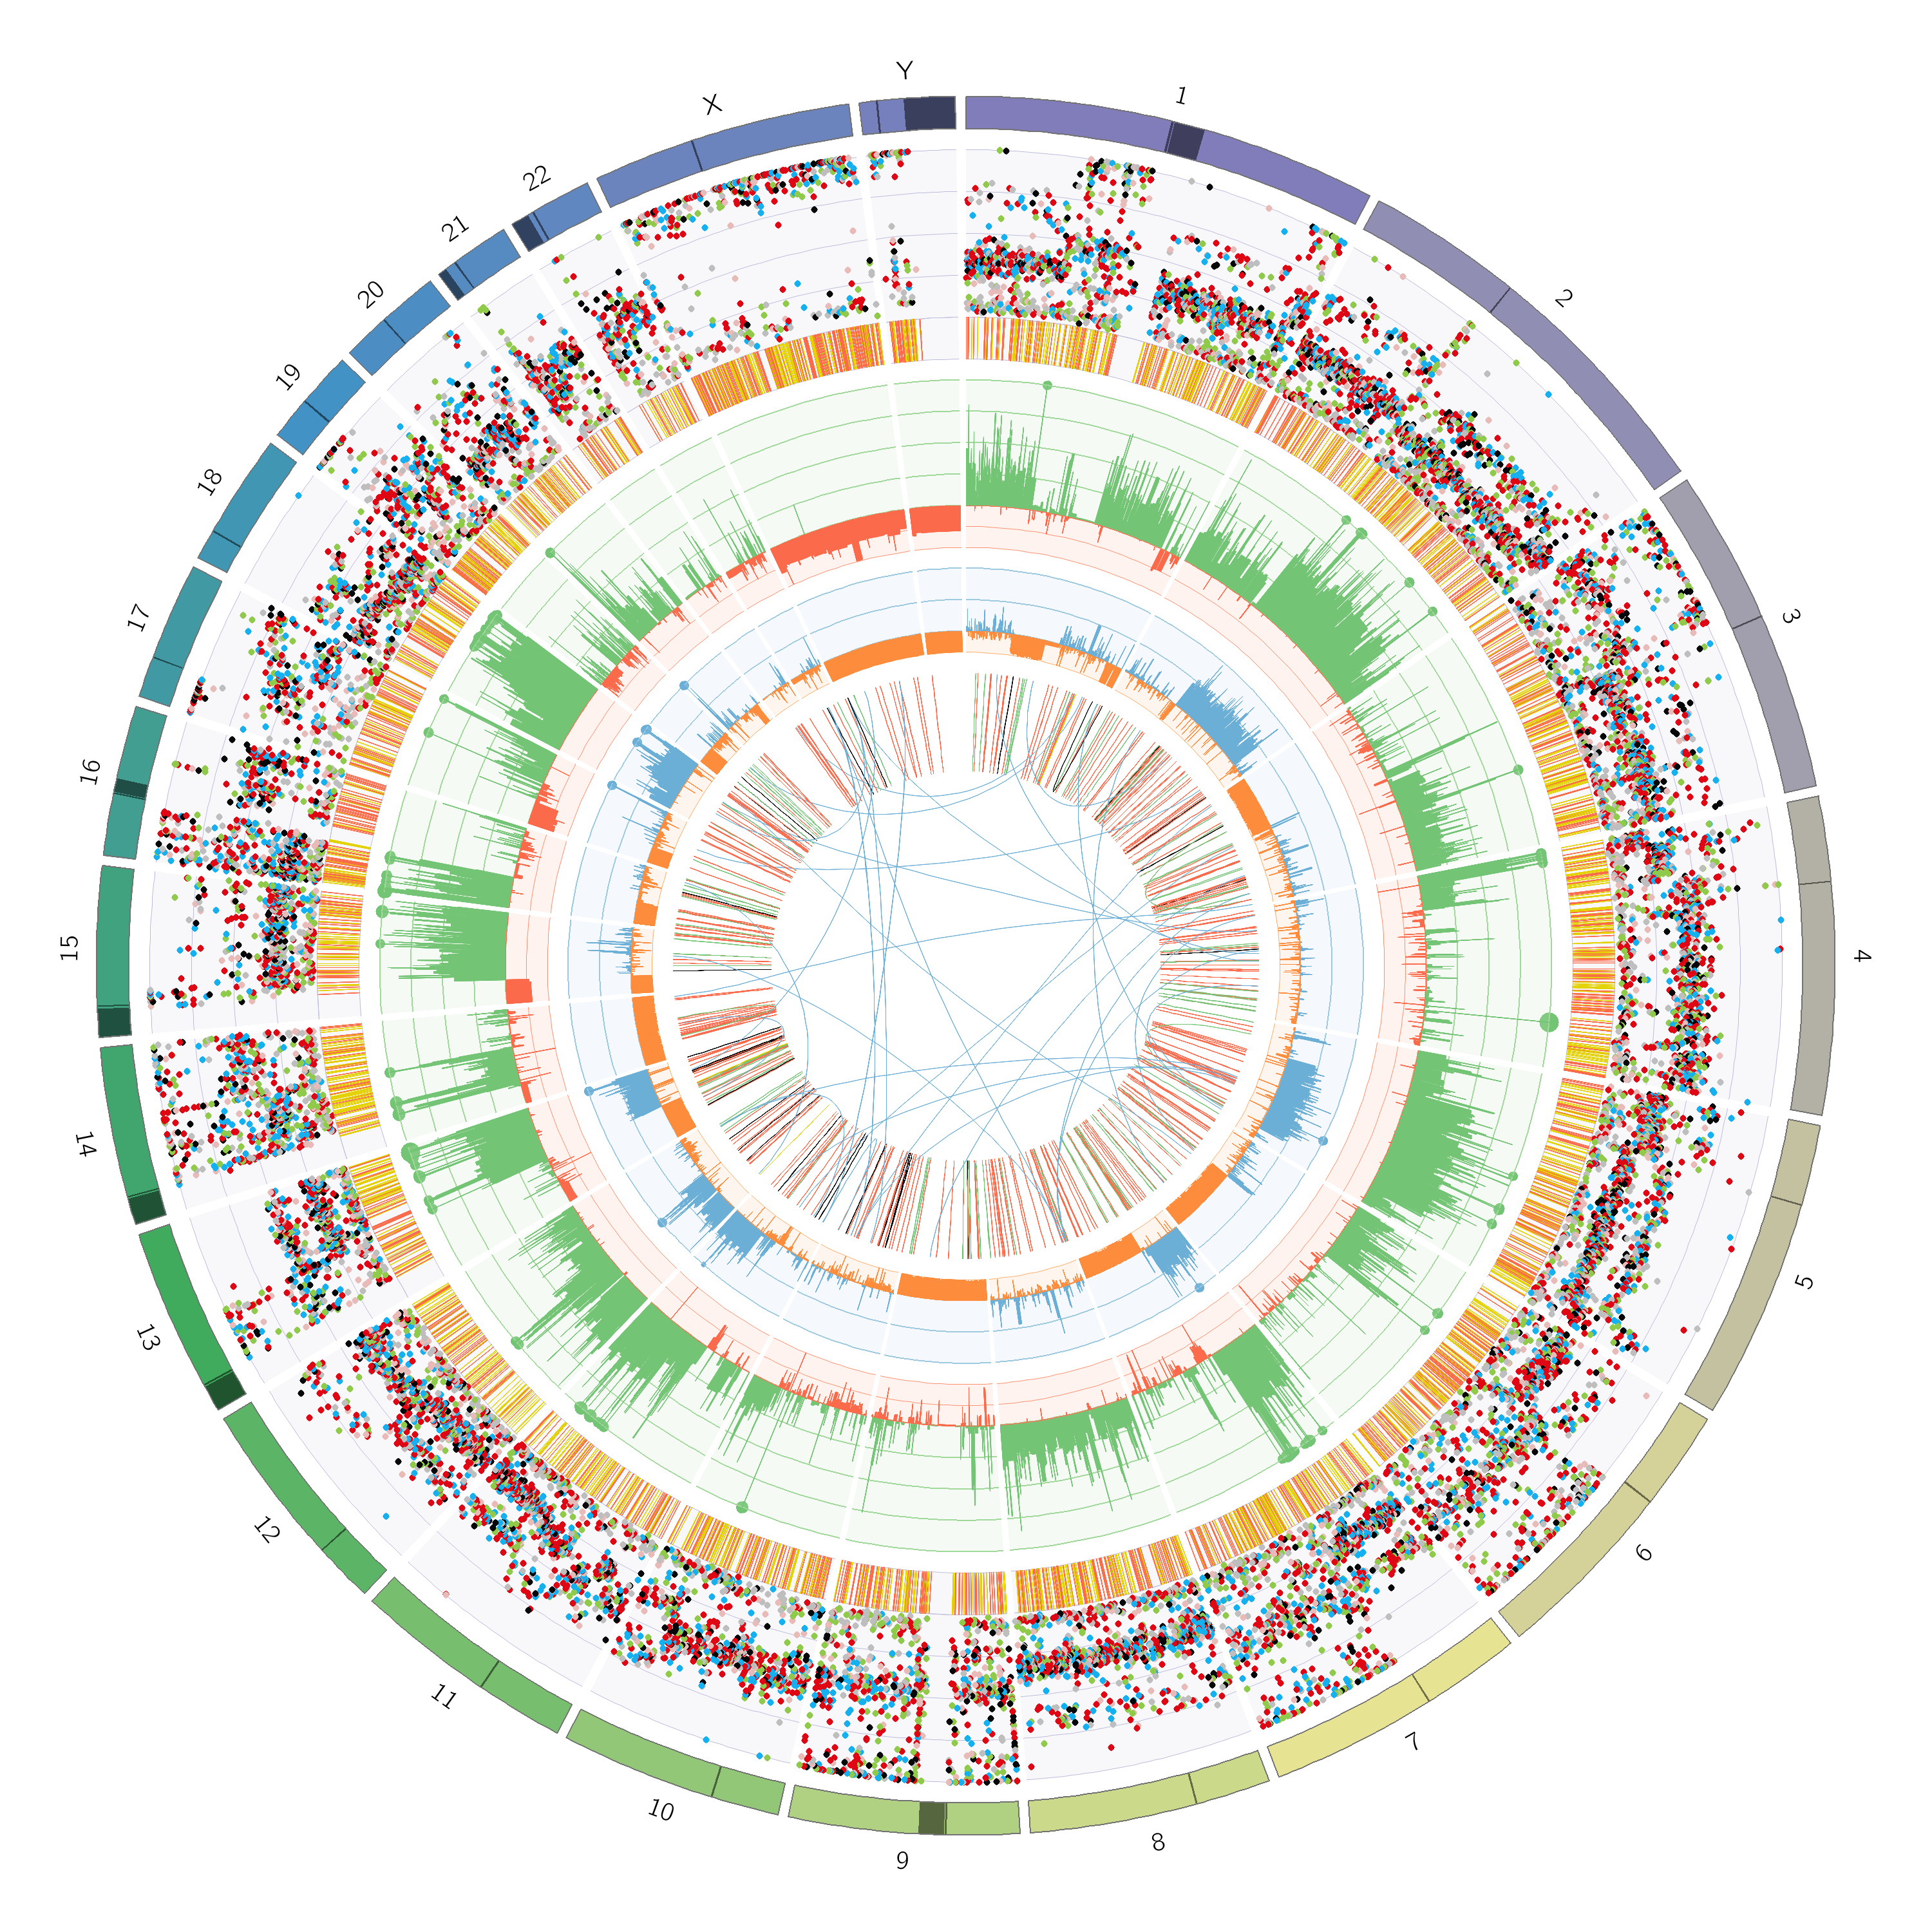
\includegraphics[width=.99\linewidth]{Figures/CASCADE/CA99/CA99-11.circos.png}
\caption[Circos plot of patient CA-A sample 11]{Circos plot of patient CA-A with somatic structural variants with allele frequency $> 0.2$: outer first ring shows the canonical chromosomes with gaps (centromere, heterochromatin,...) highlighted as darker areas; second ring visualises all somatic SNVs corrected for tumour purity and scaled from 0 to 1, the colour representing the base change of SNV like in \protect\textcite{Alexandrov2013}; vertical lines directly under the SNVs symbolise InDels, with yellow for insertions and red for deletions; the third ring shows the total copy number alterations, with green showing a copy number gain and red a loss, dots at the outer border show a copy number greater than four; the last ring shows the minor copy number, with blue depicting a gain and orange a loss, this ring allows the detection of copy number neutral changes, like loss of heterozygosity; the center shows all structural variants: translocations in blue, deletions in red, insertions in yellow, tandem duplications in green and inversions in black.} \label{fig:ca99.11circos}
\end{figure}

\todo{think about putting the circos plot on one page} %, height=.4\textheight, keepaspectratio

\Autoref{fig:ca99.11circos,fig:ca99.26circos,fig:ca99.41circos,fig:ca99.47circos,fig:ca99.55circos,fig:ca99.57circos,fig:ca99.59circos} show very similar copy number profiles of all tumour samples of patient CA-A, with loss of heterozygosity on almost all chromosomes apart from chromosome 5 and 9, only \autoref{fig:ca99.26circos} shows a less granular mix of gain and loss of the minor allele, which is most likely due to the lower tumour purity of the sample. However, all samples exhibit high copy number gain levels consistent with whole genome duplication (\Autoref{tab:ca99wgsSamples,tab:ca99cnv}). All samples show a copy number gain in chromosome 7 at the \textit{EGFR} locus leading to \textit{EGFR} amplification (min: 3.9 max: 9.9), which is a known resistance mechanism to Levantinib \cite{Jin2021} and was therefore most likely a result of previous treatment (\autoref{fig:ca99timeline}). Just as expected from the results of the Guardant360 ctDNA results leading up to the death of the patient, there is no \textit{MET} amplification present in the patient at any site\todo{Do i need more genes here?}.

With the absence of any other plausible mechanism, of SNV, SV or CNV nature, the only possible explanation of resistance to Selpercatinib in the patient are the solvent front mutations RET~G810C/R/S/V as described in \textcite{Solomon2020}. However, the autopsy revealed substantial spatial heterogeneity of the emerged resistance mechanisms within the patient which was previously unappreciated.

\begin{table}[ht]
\caption[Copy number analysis results for patient CA-A]{Copy number analysis results for patient CA-A: results are taken from the best fit result of PURPLE; WG: whole genome}\label{tab:ca99cnv}
\centering
\rowcolors{2}{gray!15}{white}
\begin{tabular}{|c|c|c|c|c|}
\toprule
\hline
 \rowcolor{gray!50}
\textbf{Sample number} & \textbf{purity} & \textbf{ploidy} & \textbf{polyclonal \%} & \textbf{WG duplication}\\
\hline
 11 & \num{0.73} &	 \num{2.86} &	\num{29.75} & \cellcolor{white}	\\
 26 & \num{0.61} & \num{3.00} & \num{26.57} & \cellcolor{white} \\
 31 & \num{0.21} & \num{5.40} & \num{49.86} & \cellcolor{white} \\
 41 & \num{0.28} & \num{4.30} & \num{42.43} & \cellcolor{white} \\
 47 & \num{0.46} & \num{2.86} & \num{29.72} & \cellcolor{white} \\
 55 & \num{0.38} & \num{2.86} & \num{38.41} & \cellcolor{white} \\
 57 & \num{0.61} & \num{3.00} & \num{28.55} & \cellcolor{white} \\
 59 & \num{0.69} & \num{2.60} & \num{37.11} & \cellcolor{white}\multirow{-8}{*}{True} \\
 \hline
\bottomrule
\end{tabular}
\end{table} 

With the high percentage of likely sub-clonality of samples (\Autoref{tab:ca99cnv}) we used PhylogicNDT to

\todo[inline]{add the phylogicNDT results}

%we clear all floats before we go to the next patient
\cleardoublepage


%%%%%%%%%%%%%%%%%%%%%%%%%%%%%%%%%%%%%%%%%%%%%%%%%%%%%%%%%%%%%%%%%%%%%%%%%%%%%%%%%%%%%%%
%                               Patient CA51                                          %
%%%%%%%%%%%%%%%%%%%%%%%%%%%%%%%%%%%%%%%%%%%%%%%%%%%%%%%%%%%%%%%%%%%%%%%%%%%%%%%%%%%%%%%


\subsection{Patient CA-I}
\label{cascade-sec:CA51}

This 56 year old female never smoker presented with \textit{EGFR} exon 19 deletion positive lung cancer in stage \todo{which stage} with metastatic involvement. After initially good response with Gefitinib treatment, the patient showed progressive nodal disease and was moved to Carboplatin/Gemcitabine chemotherapy with mixed response. After the change to Afatinib small intra-cranial metastases were detected and biopsy of the parasternal mass revealed small cell transformation in addition to the EGFR~T790M resistance mutation. Subsequent treatment change to Carboplatin/Etoposide as well as CAV (cyclophosphamide, doxorubicin, vincristine) and finally Nivolumab were not successful and the patient died 40 months after diagnosis (\autoref{fig:ca51timeline}).

\begin{figure}[ht]
	\centering
	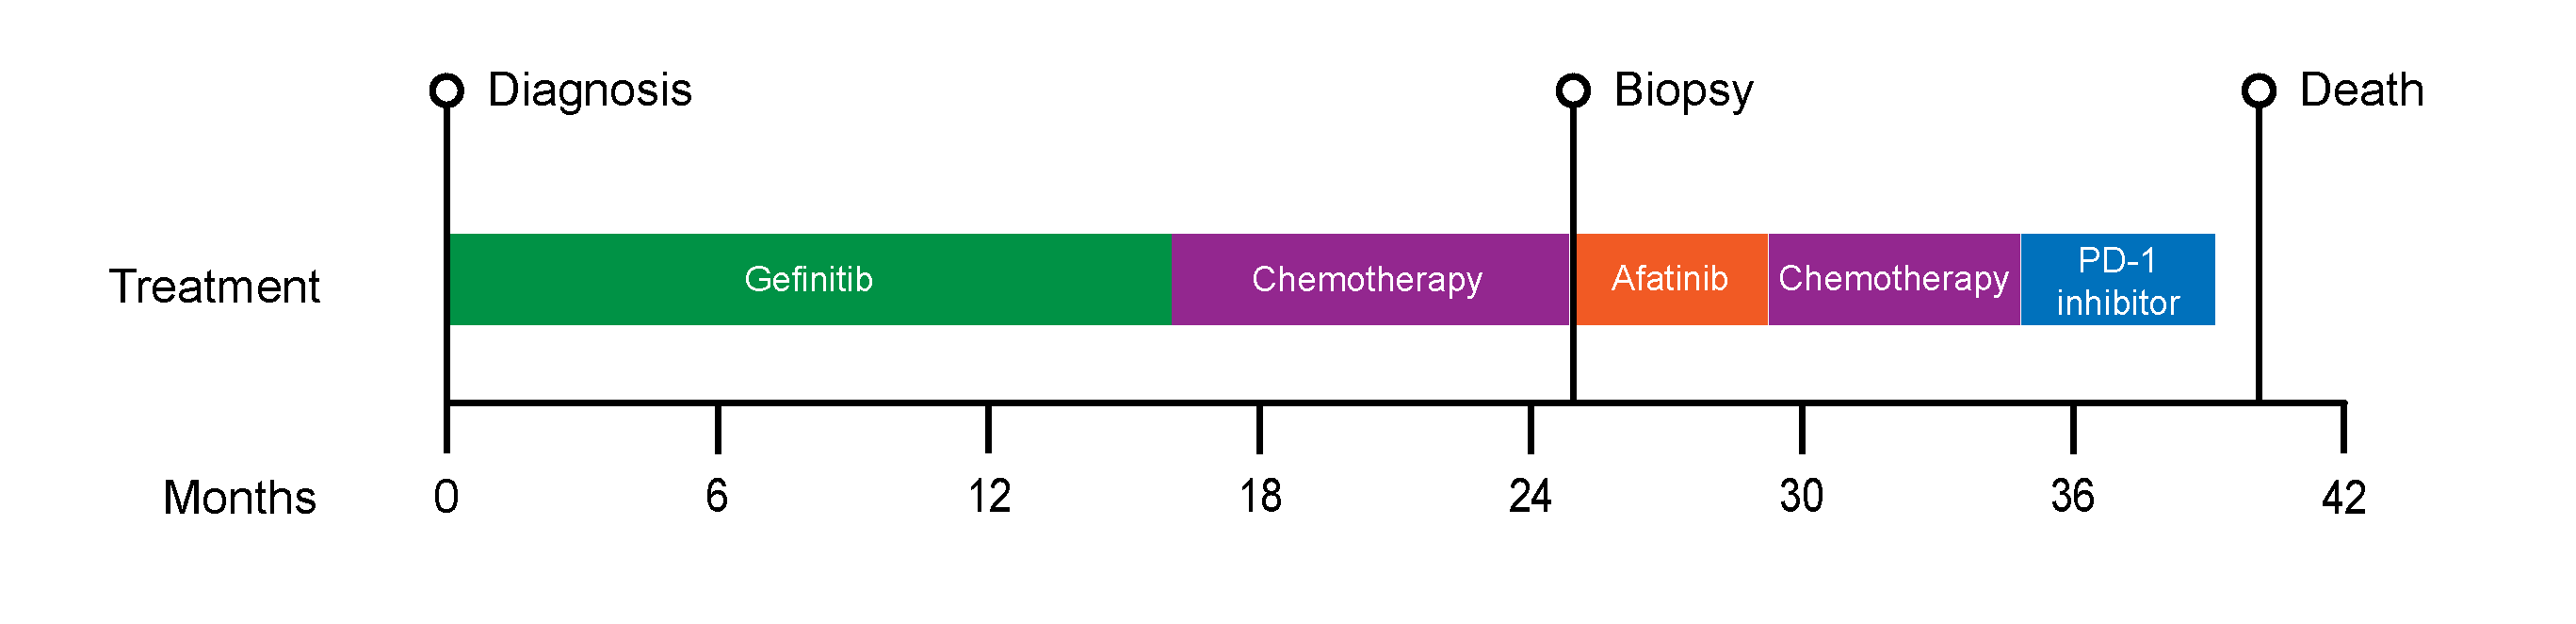
\includegraphics[width=.99\linewidth]{Figures/CASCADE/CA51/CA-I_timeline}
	\caption[Timeline of patient CA-I from diagnosis until death]{Timeline of patient CA-I from diagnosis until death: Diagnostic biopsy detected EGFR exon 19 deletion lung adenocarcinoma; Second biopsy after 24 months revealed additional EGFR~T790M mutation and small cell transformation} \label{fig:ca51timeline}
\end{figure}

At autopsy six lesions and one blood sample were collected and biobanked (\autoref{fig:cas51schematic}). After quality assessment by pathology with H\& E stain, all autopsy samples and the initial diagnostic biopsy were sequenced as WES (\autoref{tab:ca51wesSamples}) and analysed with the standard workflow (\autoref{cascade-sec:workflow}). The secondary small cell confirmation biopsy at 29 months did not contain enough tissue for sequencing.

\begin{figure}[ht]
	\centering
	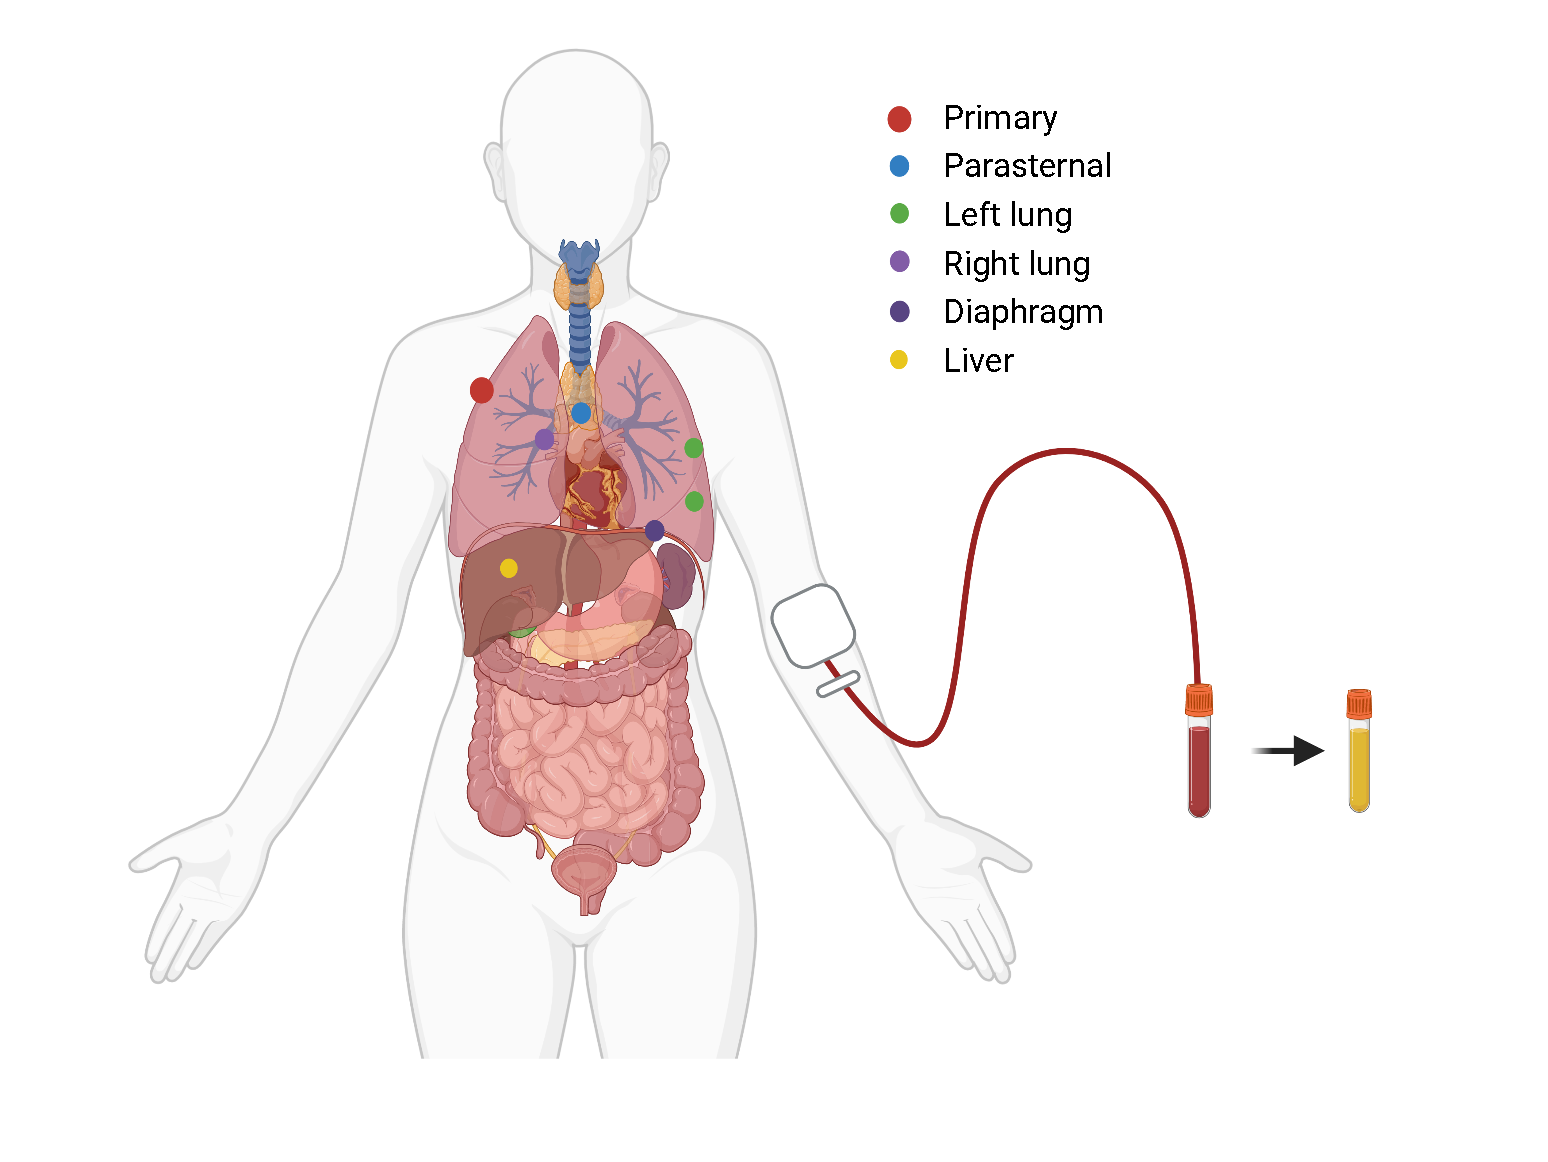
\includegraphics[width=.99\linewidth]{Figures/CASCADE/CA51/CA-I_schematic_CA51_organColours}
	\caption[Schematic of tumour lesions in patient CA-I]{Schematic of tumour lesions in patient CA-I: Primary diagnostic sample shown in red; All six autopsy samples were coloured by organ they were collected from: Parasternal (1), left lung (2), right lung (1), diaphragm (1), liver (1); Additionally a post mortem blood sample was taken} \label{fig:cas51schematic}
\end{figure}


\begin{table}[ht]
	\caption[Autopsy samples sequenced for patient CA-I]{Autopsy samples sequenced for patient CA-I: Sample number is the internal sample collection during CASCADE autopsy, the organ of the sample, the fraction of tumour cell from H\& E stain and the pathology of the tumour sample. Dx: diagnostic sample} \label{tab:ca51wesSamples}
	\centering
	\rowcolors{2}{gray!15}{white}
	\begin{tabular}{|c|c|c|c|c|}
	\toprule
	\hline
 	\rowcolor{gray!50}
\textbf{Sample number} & \textbf{Organ} & \textbf{H \& E} & \textbf{Type}\\
	\hline
 Dx & right VATS & - &  adenocarcinoma \\
 557 & parasternal mass & 0.9 & \cellcolor{gray!15} \\
 559 & left diaphragm & 0.9 & \cellcolor{gray!15} \\
 566 & right liver lobe & 0.6 & \cellcolor{gray!15} \\
 573 & right hilar lymph node & 0.9 & \cellcolor{gray!15} \\
 579 & left lung lobe & 0.8 & \cellcolor{gray!15} \\
 583 & left pleura & 0.9 & \cellcolor{gray!15}\multirow{-6}{*}{small cell} \\
 	\hline
	\bottomrule
	\end{tabular}
\end{table} 


Somatic variant calling showed very little genetic heterogeneity. The original \textit{EGFR} exon 19 deletion was present in all sequenced samples from the diagnostic to the 40 months later autopsy samples. No other protein altering somatic mutations were detected at a purity corrected allele frequency $\geq 0.33$. While the diagnostic sample presented with TERT~H687Q at 25\% VAF with sufficient local copy number amplification, none of the autopsy samples showed any support for this variant. Generally, the number of somatic protein altering SNVs and InDels (min:988 max: 1236 mean: 1090.5)  is very close to the average lung adenocarcinoma with an observed tumour mutational burden of 18.75 \cite{Alexandrov2013}. 
In contrast, the diagnostic sample showed a much higher number of mutations, which we attribute to the formalin-fixed paraffin-embedded (FFPE) preservation, which is known to cause DNA damage \cite{Do2015}. This DNA damage could have led to a higher rate of called somatic variants (\autoref{fig:ca51numVars}). In order to appreciate the relationship of the autopsy samples, we removed the diagnost sample from the phylogenetic analysis. The full phylogeny can be seen in \autoref{fig:ca51phyloWithDx}. The phylogeny of SNVs and InDels shows no internal hierarchical structure, but rather shows that both stem of tumour initiation and additional private mutations accumulated during the disease progression are approximatly equal in number, with the stem being slightly longer. Only a very limited amount of somatic variants are shared between cancer samples, which are not part of the initial stem (\autoref{fig:ca51phylo}). Which is consistent with the clinical history, where there never was any remission, but only mixed response of already established lesions.

\begin{figure}[ht]
	\centering
	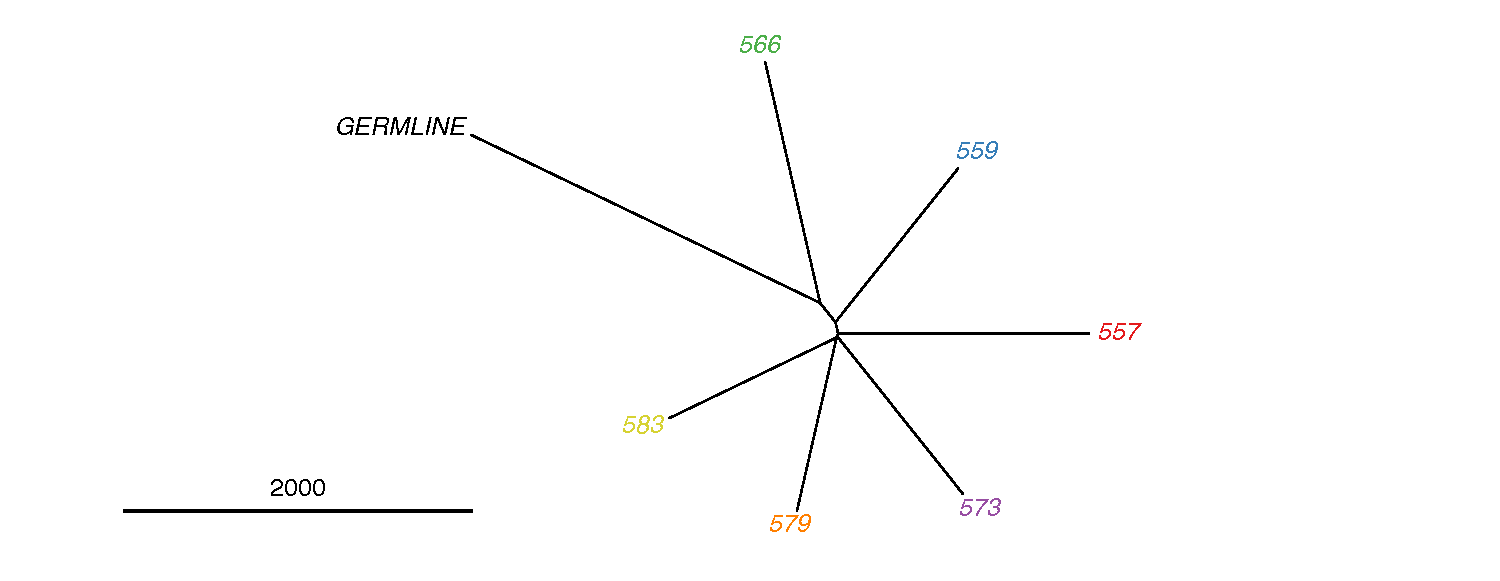
\includegraphics[width=.99\linewidth]{Figures/CASCADE/CA51/CA51phyloAutopsy.pdf}
	\caption[Phylogeny of autopsy samples from patient CA-I]{Phylogeny of autopsy samples from patient CA-I; reconstructed with all somatic SNVs and InDels. The phylogeny with diagnostic sample can be found in \protect\autoref{ca51phyloWithDx}} \label{fig:ca51phylo}
\end{figure}

Due to the pathology information of small cell transformation, we could highlight an intronic \textit{TP53} mutations, which is present at almost 100\% VAF in all autopsy samples. However the same variant was also found in the diagnostic sample, which was reportedly adenocarcinoma. The variant was therefore not sufficient to drive the transformation, but could have been a predisposition for the patient.



When comparing the diagnostic sample with the samples at autopsy the most striking difference is the lower overall copy number gain. The cause of this difference is  the amplified minor allele in the diagnostic sample, which is almost completely absent in all autopsy samples. However this amplification in the diagnostic sample could be rooted in the FFPE DNA damage combined with the lower purity of the sample, which in term at used as a sign of amplification of the minor allele after purity correction through sequenza. 
The consistent feature between all samples, diagnostic and autopsy, is the loss of heterozygosity on chromosomes 2, 4, 10 through 13, and 19. With consistent copy number gains at the end of chromosome 1, 3 and 7 and all of chromosome 5 and 6.
The high amplification of chromosome 7 is consistent with the origin of \textit{EGFR} driven primary tumour and the copy number loss of the start of chromosome 17 for all autopsy samples, but only a loss of heterozygosity in the primary sample is consistent with the genetic prerequisites for small cell transformation. (\autoref{fig:ca51.dxcircos} vs. \Autoref{fig:ca51.557circos,fig:ca51.559circos,fig:ca51.566circos,fig:ca51.573circos,fig:ca51.579circos,fig:ca51.583circos} and \autoref{tab:ca51cnv}).
\todo{what more do i write here? other drivers?}


\begin{figure}[ht]
\centering
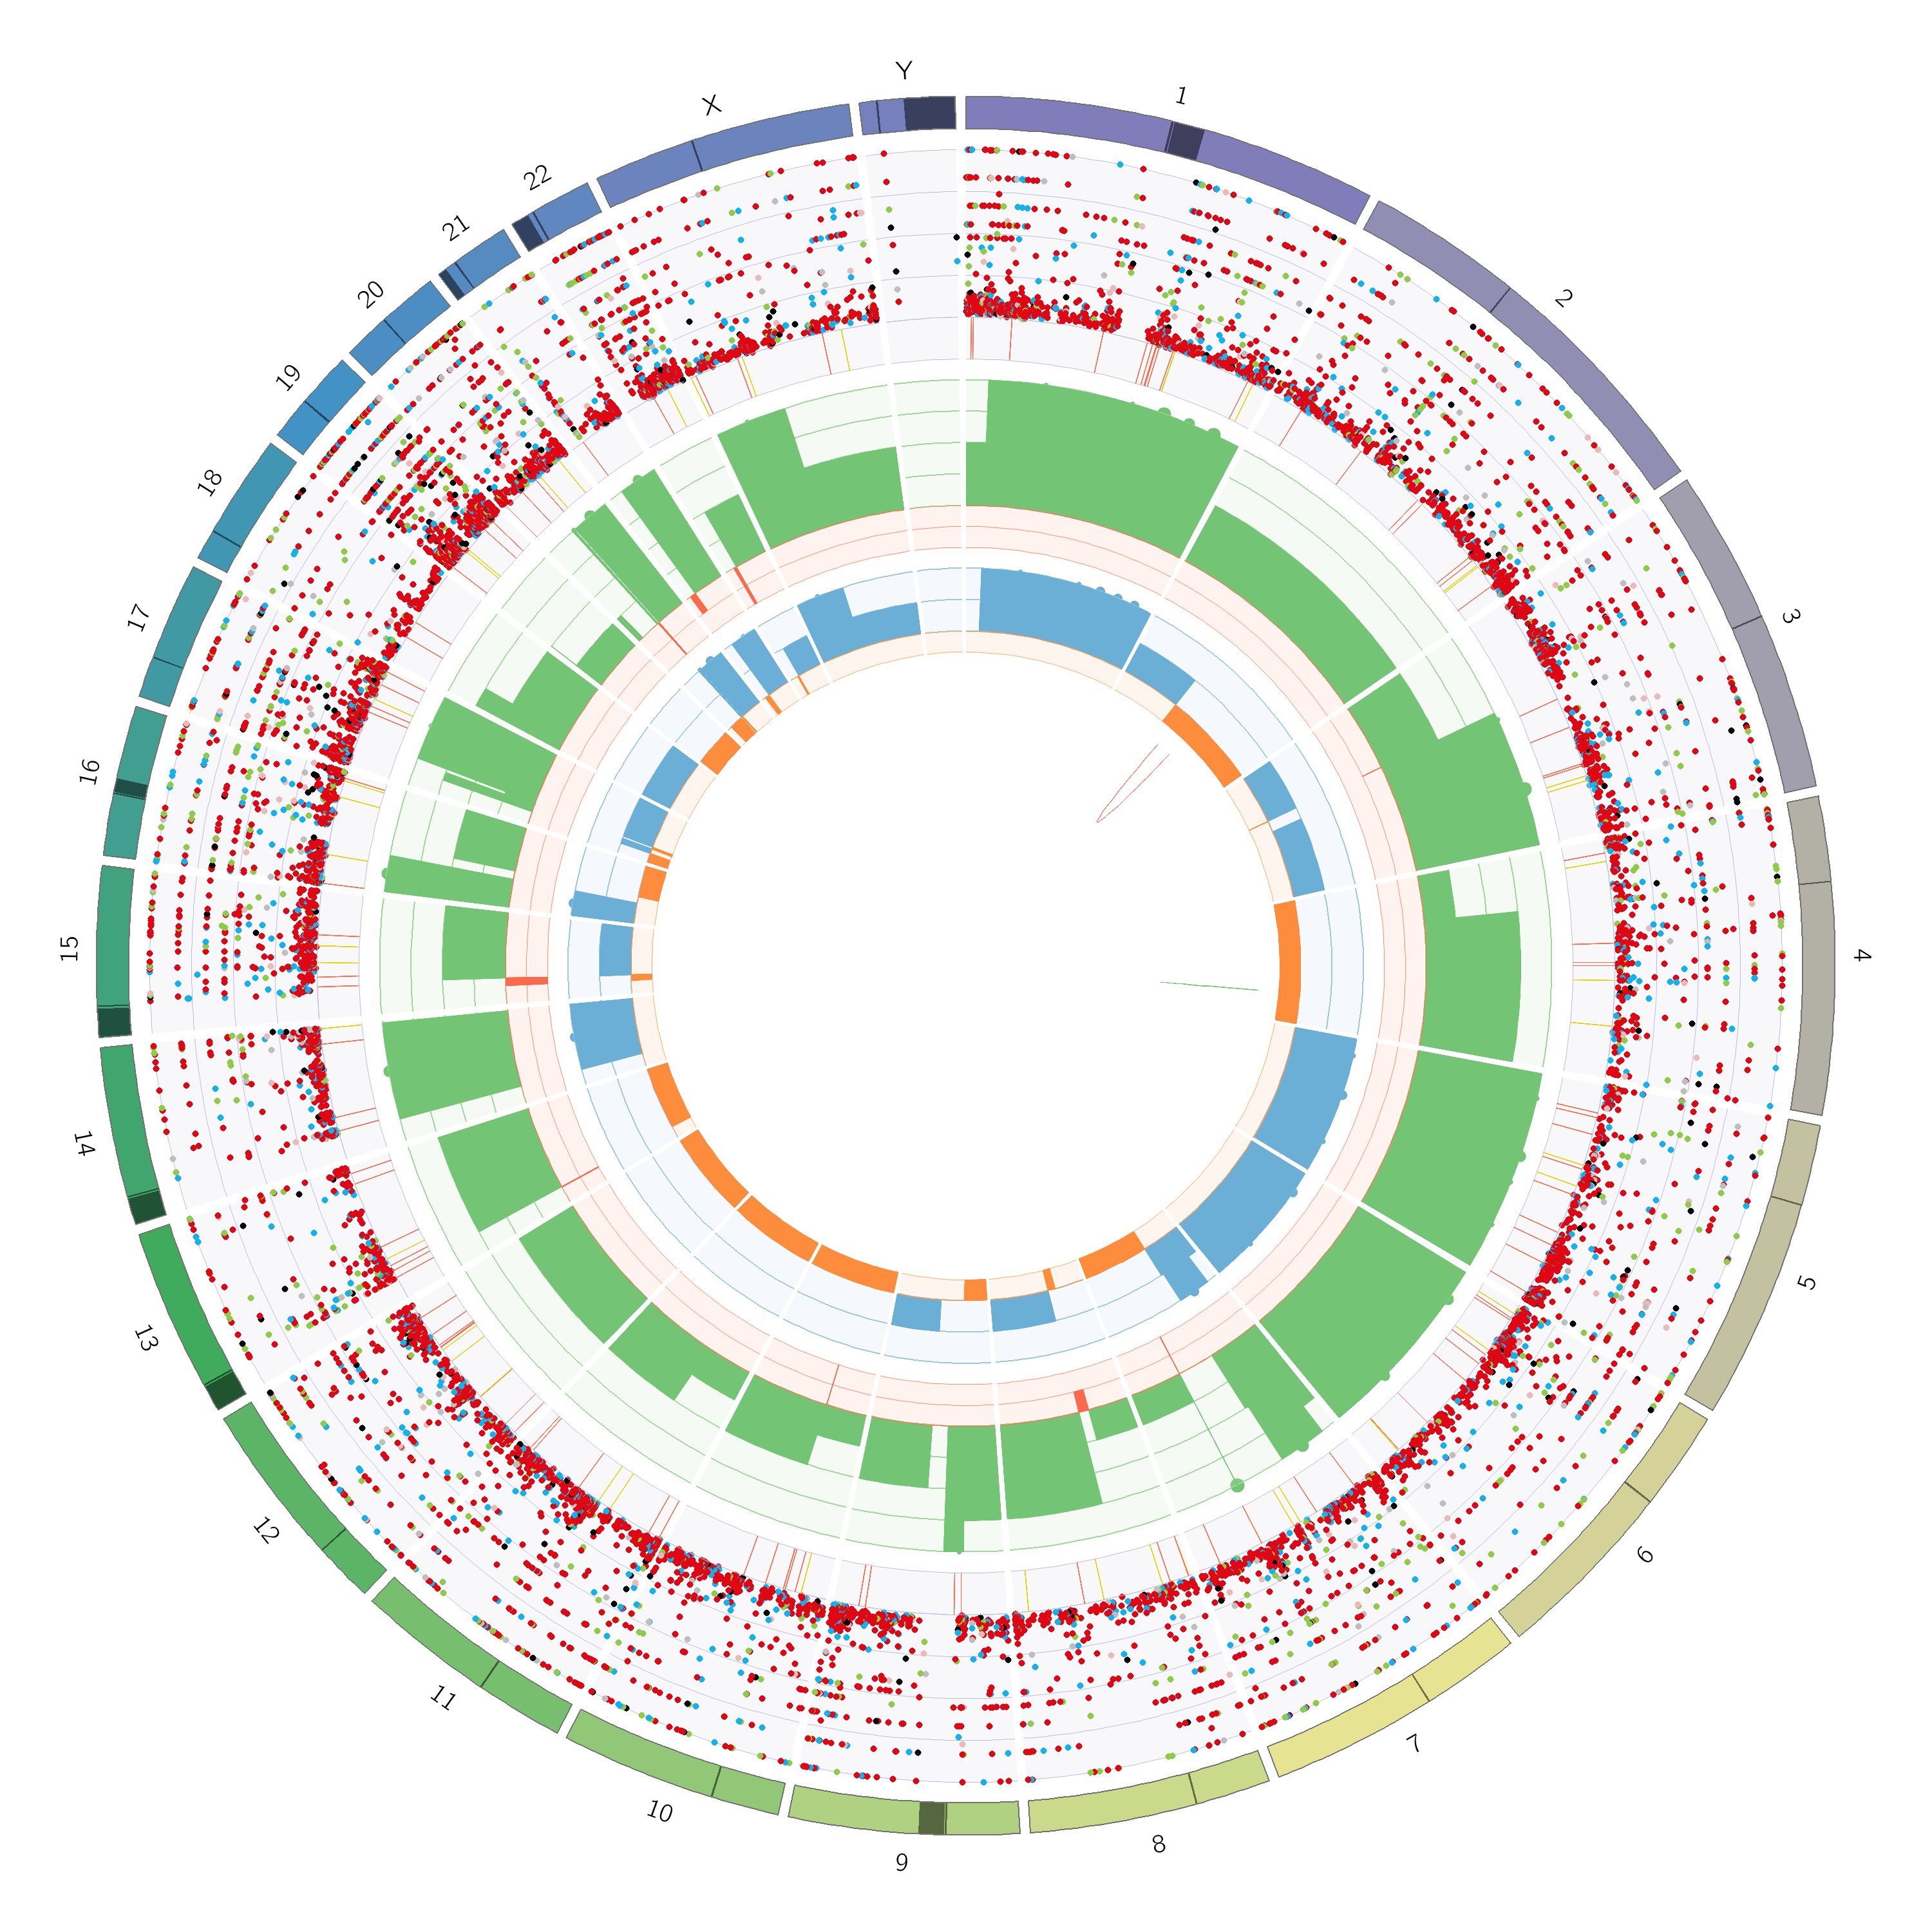
\includegraphics[width=.99\linewidth]{Figures/CASCADE/CA51/CA51-Ep12P3369.circos.png}
\caption[Circos plot of patient CA-I sample dx]{Circos plot of patient CA-I sample dx with somatic structural variants with allele frequency $> 0.2$: outer first ring shows the canonical chromosomes with gaps (centromere, heterochromatin,...) highlighted as darker areas; second ring visualises all somatic SNVs corrected for tumour purity and scaled from 0 to 1, the colour representing the base change of SNV like in \protect\textcite{Alexandrov2013}; vertical lines directly under the SNVs symbolise InDels, with yellow for insertions and red for deletions; the third ring shows the total copy number alterations, with green showing a copy number gain and red a loss, dots at the outer border show a copy number greater than four; the last ring shows the minor copy number, with blue depicting a gain and orange a loss, this ring allows the detection of copy number neutral changes, like loss of heterozygosity; the center shows all structural variants: translocations in blue, deletions in red, insertions in yellow, tandem duplications in green and inversions in black.} \label{fig:ca51.dxcircos}
\end{figure}


\begin{figure}[ht]
\centering
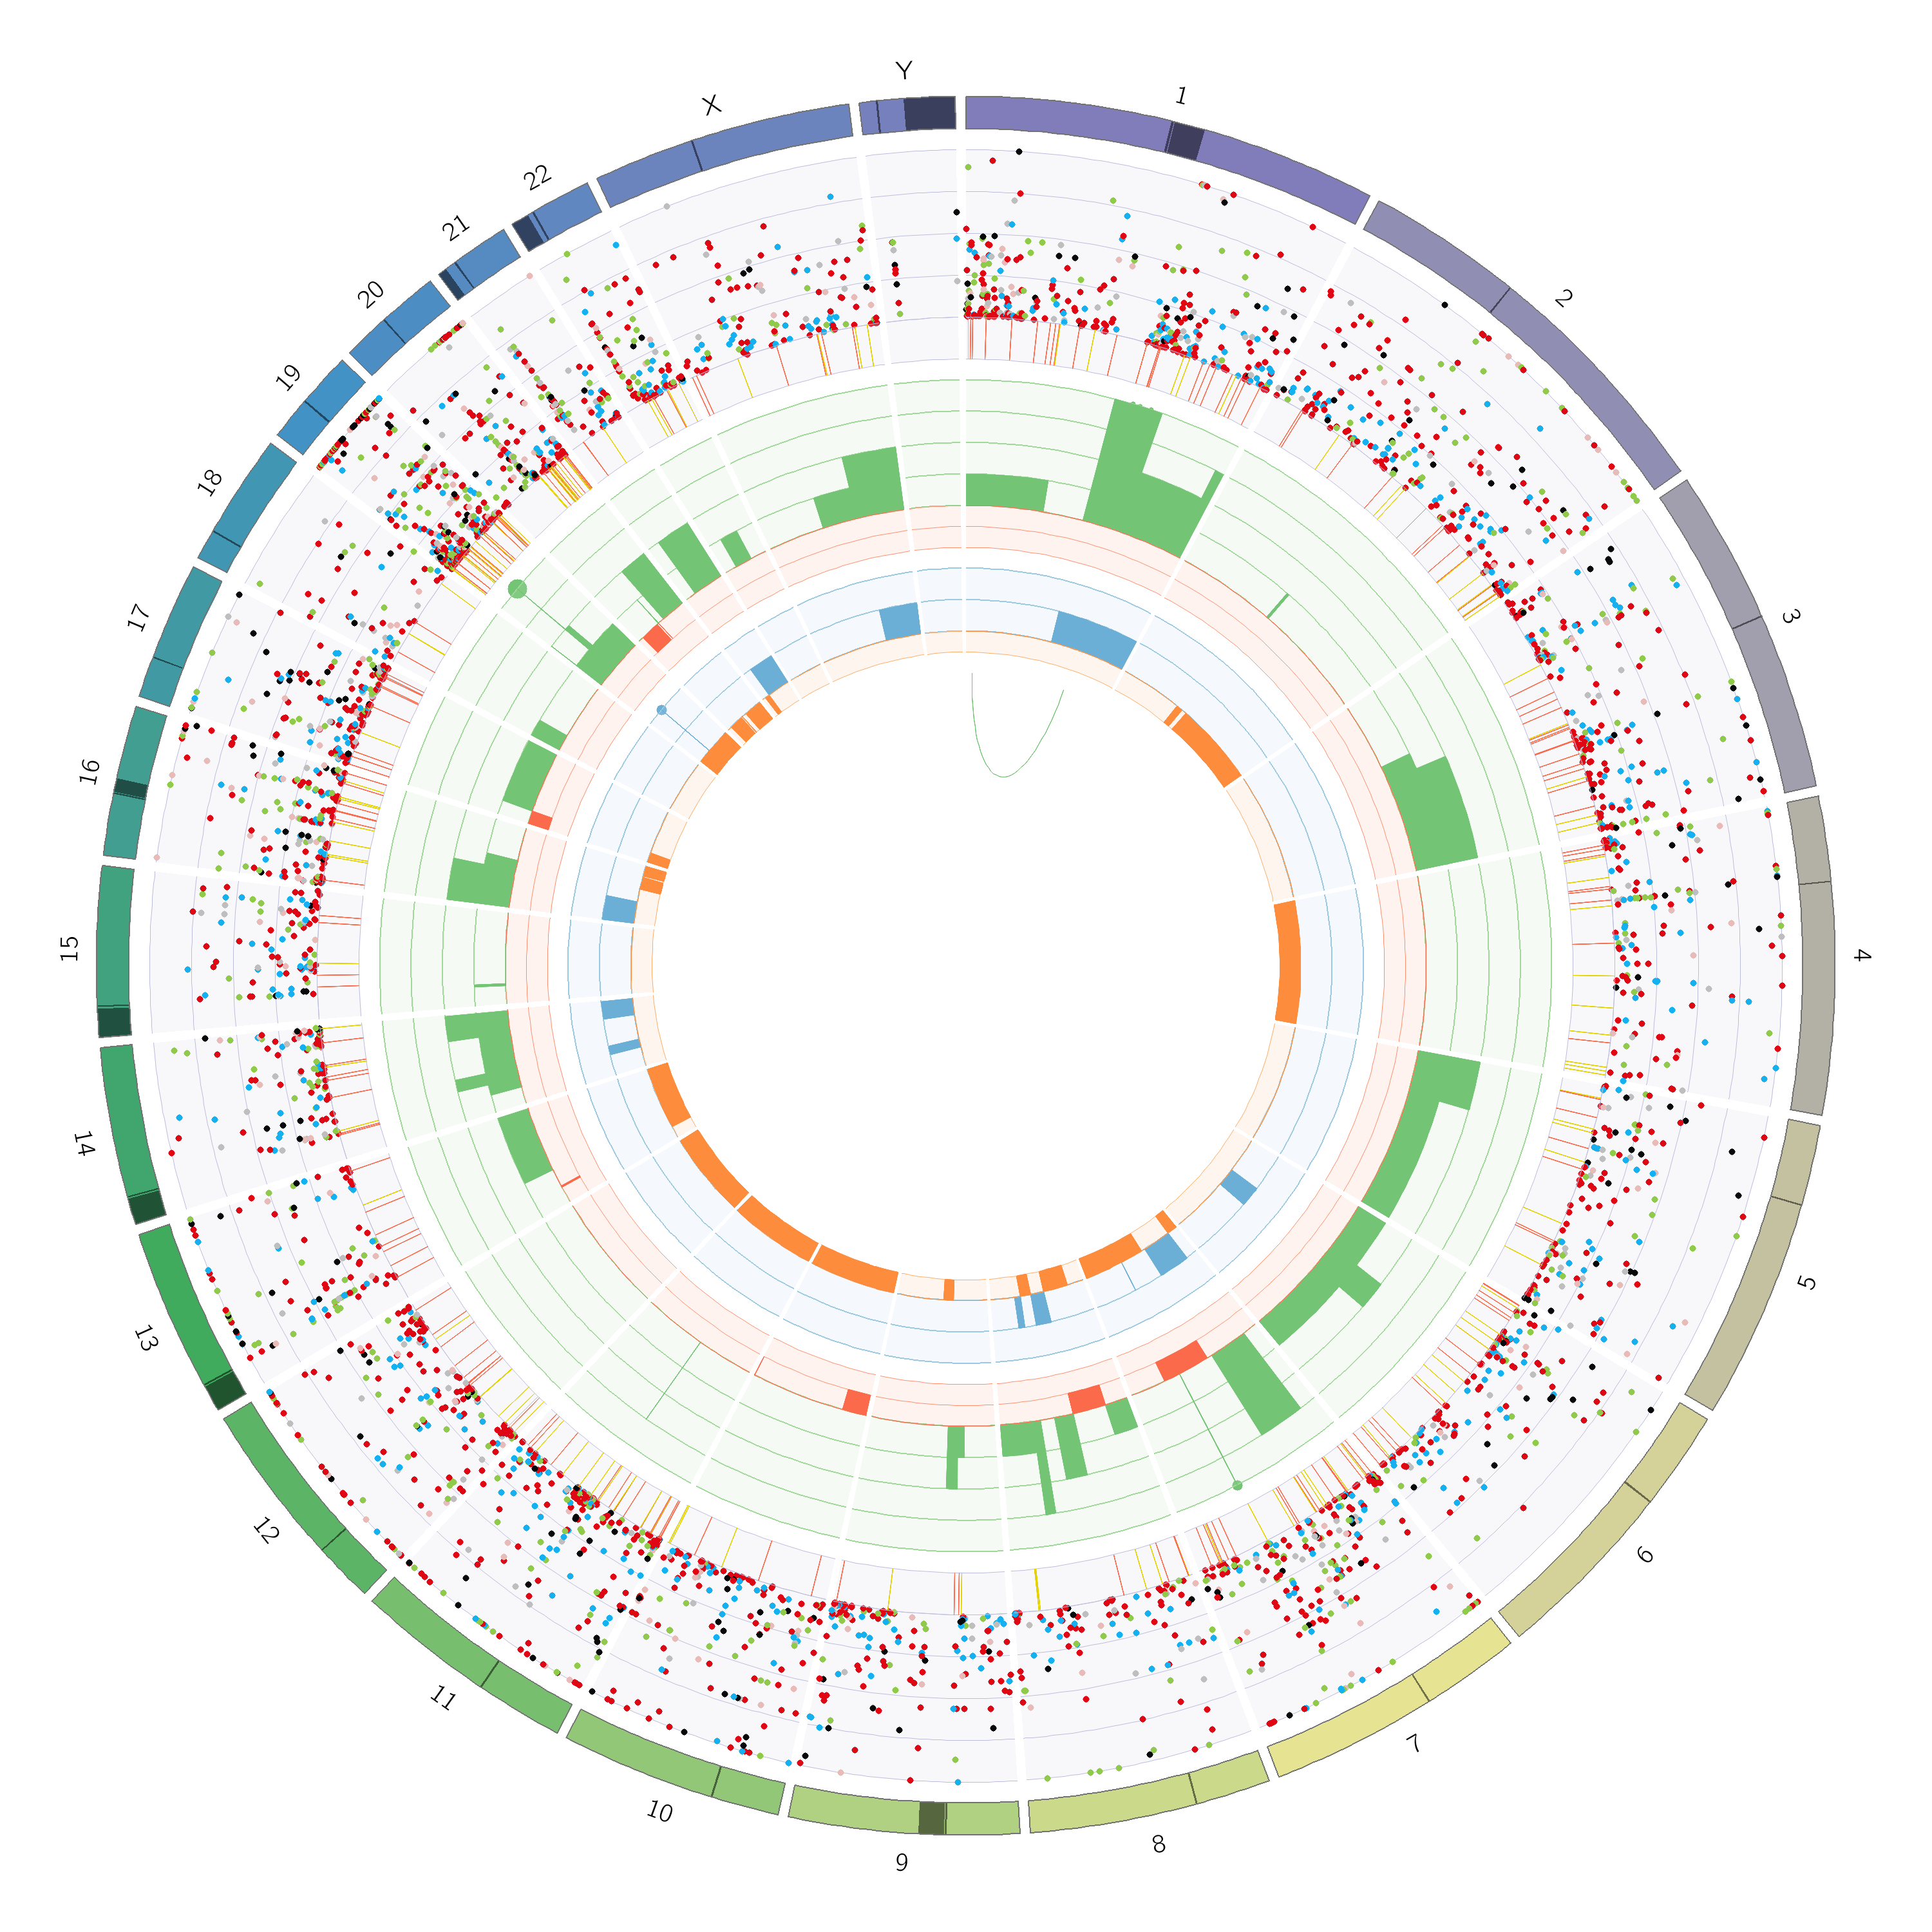
\includegraphics[width=.99\linewidth]{Figures/CASCADE/CA51/CA51-557.circos.png}
\caption[Circos plot of patient CA-I sample 557]{Circos plot of patient CA-I sample 557 with somatic structural variants with allele frequency $> 0.2$: outer first ring shows the canonical chromosomes with gaps (centromere, heterochromatin,...) highlighted as darker areas; second ring visualises all somatic SNVs corrected for tumour purity and scaled from 0 to 1, the colour representing the base change of SNV like in \protect\textcite{Alexandrov2013}; vertical lines directly under the SNVs symbolise InDels, with yellow for insertions and red for deletions; the third ring shows the total copy number alterations, with green showing a copy number gain and red a loss, dots at the outer border show a copy number greater than four; the last ring shows the minor copy number, with blue depicting a gain and orange a loss, this ring allows the detection of copy number neutral changes, like loss of heterozygosity; the center shows all structural variants: translocations in blue, deletions in red, insertions in yellow, tandem duplications in green and inversions in black.} \label{fig:ca51.557circos}
\end{figure}



\begin{table}[ht]
\caption[Copy number analysis results for patient CA-I]{Copy number analysis results for patient CA-I: results are taken from the best fit result of sequenza}\label{tab:ca51cnv}
\centering
\rowcolors{2}{gray!15}{white}
\begin{tabular}{|c|c|c|c|}
\toprule
\hline
 \rowcolor{gray!50}
\textbf{Sample number} & \textbf{purity} & \textbf{ploidy} & \textbf{WG duplication}\\
\hline
 Dx  & \num{0.29} & \num{5.5} & True	\\
 557 & \num{0.93} & \num{2.6} & False \\
 559 & \num{0.96} & \num{2.6} & False \\
 566 & \num{0.69} & \num{2.7} & False \\
 573 & \num{0.94} & \num{2.6} & False \\
 579 & \num{0.95} & \num{2.6} & False \\
 583 & \num{0.95} & \num{2.6} & False \\
 \hline
\bottomrule
\end{tabular}
\end{table} 

\todo[inline]{insert phylogicNDT result, when done}

%we clear all floats before we go to the next patient
\cleardoublepage

%%%%%%%%%%%%%%%%%%%%%%%%%%%%%%%%%%%%%%%%%%%%%%%%%%%%%%%%%%%%%%%%%%%%%%%%%%%%%%%%%%%%%%%
%                               Patient CA80                                          %
%%%%%%%%%%%%%%%%%%%%%%%%%%%%%%%%%%%%%%%%%%%%%%%%%%%%%%%%%%%%%%%%%%%%%%%%%%%%%%%%%%%%%%%


\subsection{Patient CA-J}
\label{cascade-sec:CA80}

Patient CA-J was a 65 year old female never smoker, who presented with moderately differentiated lung  adenocarcinoma (Stage IIIB). Molecular pathology revealed metastatic EGFR~L858R positive disease in both the left and the right lungs, the surrounding lymph nodes, the left adrenal gland, multiple bones (T3, scalp and dura). Initial treatment with both Carboplatin/Paclitaxel and radiotherapy was halted after detection of additional brain, bone and lung lesions and changed to Erlotinib. Progressive pulmonary disease and subsequent left lung core biopsy showed an additional BRAF~V600E mutation. Treatment was adjusted to Carboplatin and Pemetrexed however disease still progressed in distant metastasis and recurred in the primary site. The patient was finally enrolled in the EVICT trial treating with both Vemurafenib and Erlotinib, which lead to stable bone metastasis after one month, but ultimately led to progression in both pulmonary and bone metastasis. The patient died 29 months after diagnosis (\autoref{fig:ca80timeline}).

\begin{figure}[ht]
\centering
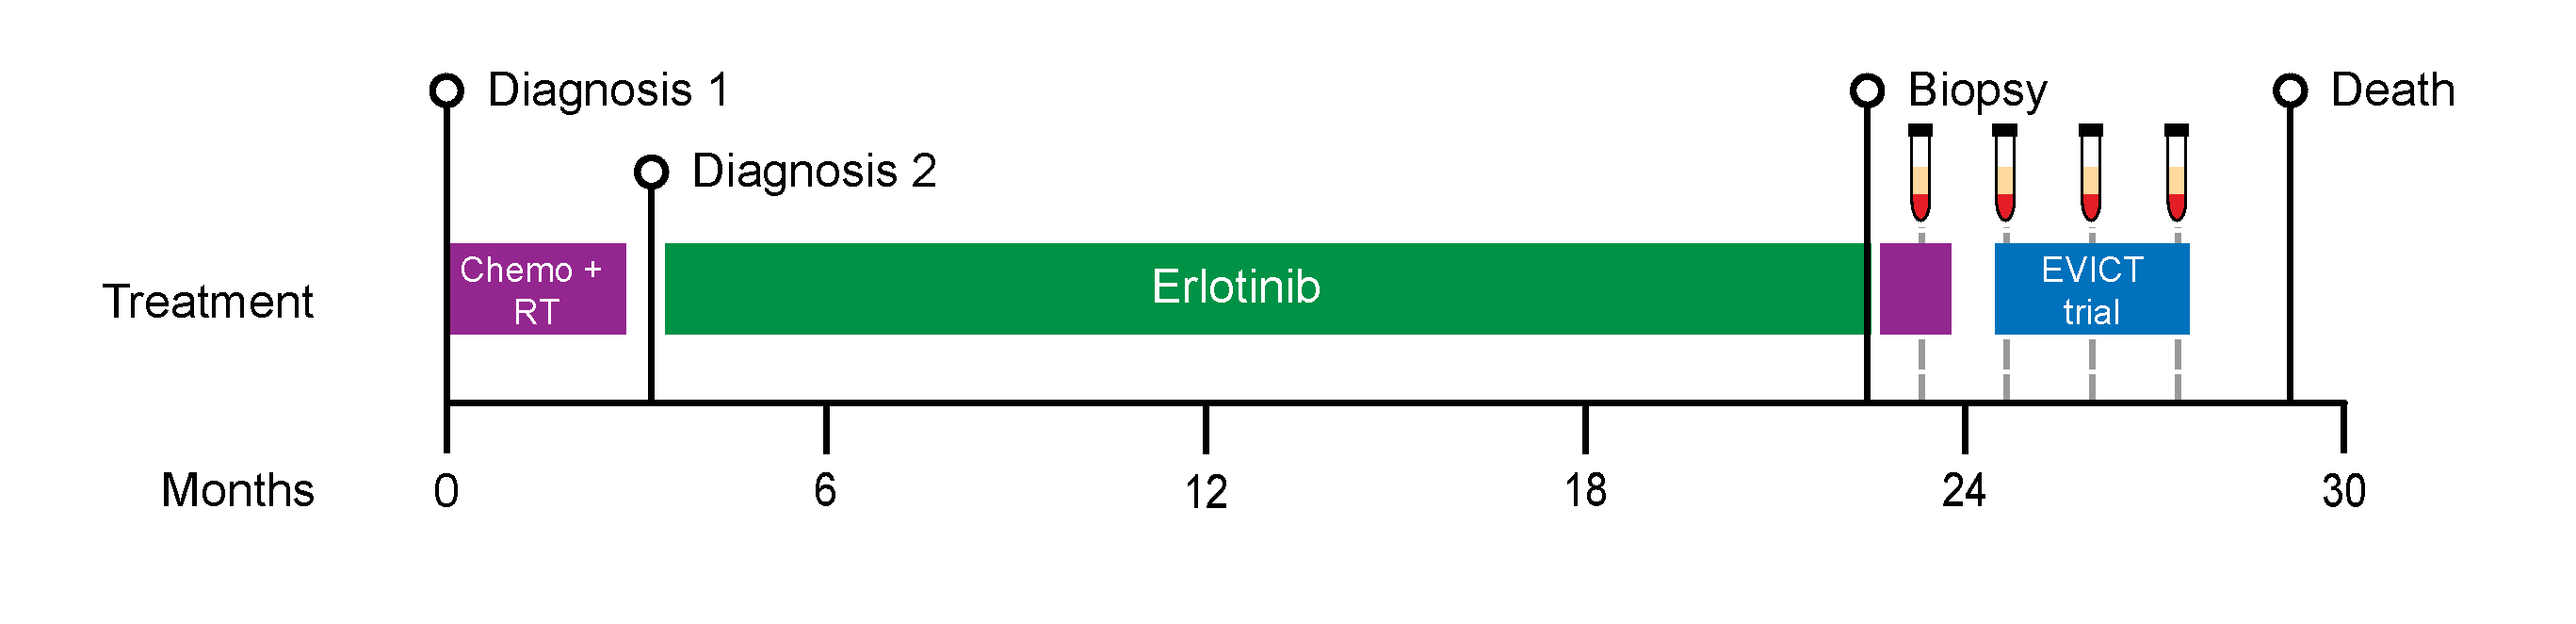
\includegraphics[width=.99\linewidth]{Figures/CASCADE/CA80/CA-J_timeline}
\caption[Timeline of patient CA-J from diagnosis until death]{Timeline of patient CA-J from diagnosis until death: Diagnostic biopsy detected EGFR~L858R positive stage IIIB lung adenocarcinoma; Second diagnosis after 3 months revealed additional brain, bone and lung metastasis with a reclassification to stage IV; Biopsy at the end of erlotinib treatment revealed additional BRAF~V600E mutation; one blood sample was taken during the second round of chemotherapy and three more during the time the patient was enrolled in the EVICT trial} \label{fig:ca80timeline}
\end{figure}





\begin{figure}[ht]
\centering
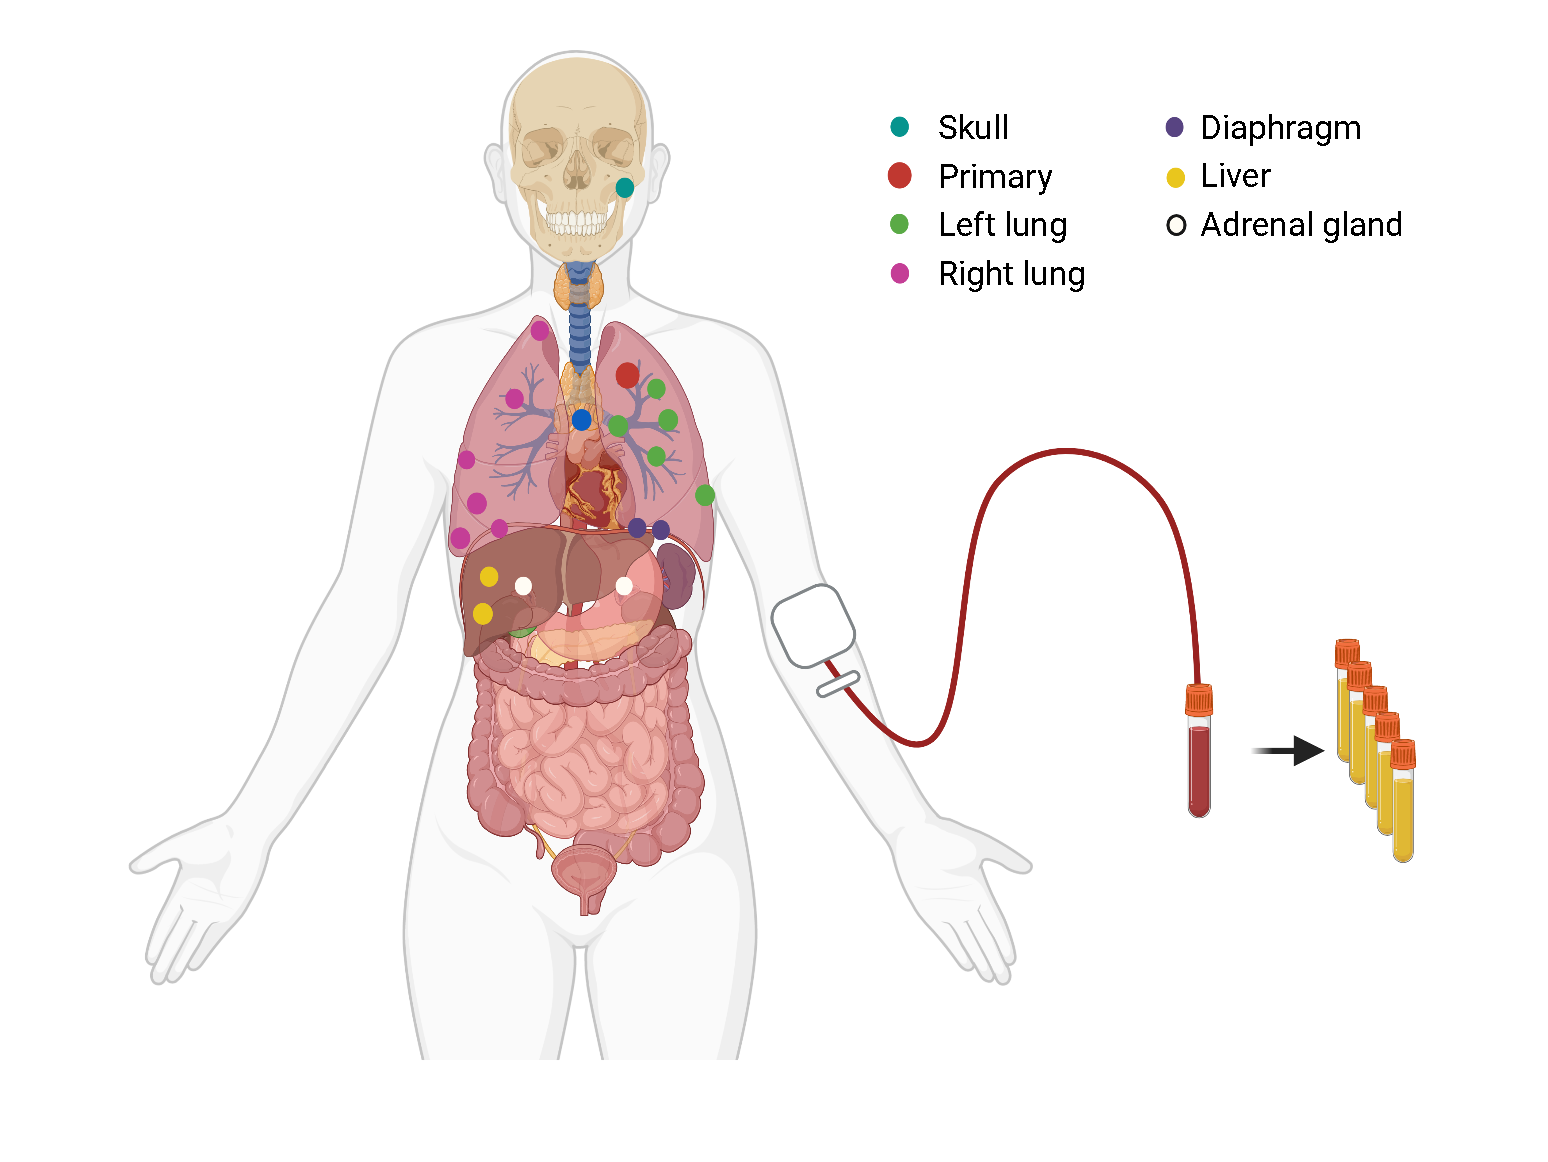
\includegraphics[width=.99\linewidth]{Figures/CASCADE/CA80/CA-J_schematic_CA80_organColours}
\caption[Schematic of analysed tumour lesions in patient CA-J]{Schematic of analysed tumour lesions in patient CA-J: Primary diagnostic sample shown in red; All 18 autopsy samples were coloured by organ they were collected from: skull (1), left lung(5), right lung (6), diaphragm (2), liver(2), adrenal gland (2); Additionally to the post mortem blood sample, four serial blood samples were taken (\protect\autoref{fig:ca80timeline})} \label{fig:cas80schematic}
\end{figure}

\begin{table}[ht]
\caption[Autopsy samples sequenced for patient CA-J]{Autopsy samples sequenced for patient CA-J: Sample number is the internal sample collection during CASCADE autopsy, the organ of the sample, the fraction of tumour cell from H\& E stain and the pathology of the tumour sample. Dx: diagnostic sample}\label{tab:ca80wgsSamples}
\centering
\rowcolors{2}{gray!15}{white}
\begin{tabular}{|c|c|c|c|c|}
\toprule
\hline
 \rowcolor{gray!50}
\textbf{Sample number} & \textbf{Organ} & \textbf{H \& E} & \textbf{Type}\\
\hline
 Dx & left lung core & - & \cellcolor{white} \\
 2 & adrenal gland & 0.5 & \cellcolor{white} \\
 20 & right lower lung & 0.7 & \cellcolor{white} \\
 24 & left upper lung & 0.9 & \cellcolor{white} \\
 28 & left middle lung & 0.5 & \cellcolor{white} \\
 32 & right upper lung & 0.5 & \cellcolor{white} \\
 42 & base of skull & 0.4 & \cellcolor{white}\multirow{-7}{*}{adenocarcinoma} \\
 \hline
\bottomrule
\end{tabular}
\end{table} 


\todo[color=red,inline]{write about somatic variant calling}



\todo[color=red,inline]{Add circos plots and write about the CNV analysis}

\begin{table}[ht]
\caption[Copy number analysis results for patient CA-J]{Copy number analysis results for patient CA-J: results are taken from the best fit result of PURPLE; WG: whole genome}\label{tab:ca80cnv}
\centering
\rowcolors{2}{gray!15}{white}
\begin{tabular}{|c|c|c|c|c|}
\toprule
\hline
 \rowcolor{gray!50}
\textbf{Sample number} & \textbf{purity} & \textbf{ploidy} & \textbf{polyclonal \%} & \textbf{WG duplication}\\
\hline
 2  & \num{0.24} & \num{2.00} & \num{15.72} & False	\\
 20 & \num{0.40} & \num{4.80} & \num{44.62} & \cellcolor{gray!15} \\
 24 & \num{0.73} & \num{3.70} & \num{32.41} & \cellcolor{gray!15} \\
 28 & \num{0.18} & \num{3.90} & \num{42.62} & \cellcolor{gray!15} \\
 32 & \num{0.25} & \num{4.75} & \num{49.71} & \cellcolor{gray!15} \\
 42 & \num{0.52} & \num{3.35} & \num{42.16} & \cellcolor{gray!15}\multirow{-5}{*}{True} \\
 \hline
\bottomrule
\end{tabular}
\end{table} 


%we clear all floats before we go to the next patient
\cleardoublepage

%%%%%%%%%%%%%%%%%%%%%%%%%%%%%%%%%%%%%%%%%%%%%%%%%%%%%%%%%%%%%%%%%%%%%%%%%%%%%%%%%%%%%%%
%                               Patient CA82                                          %
%%%%%%%%%%%%%%%%%%%%%%%%%%%%%%%%%%%%%%%%%%%%%%%%%%%%%%%%%%%%%%%%%%%%%%%%%%%%%%%%%%%%%%%


\subsection{Patient CA-K}
\label{cascade-sec:CA82}

\begin{figure}[ht]
\centering
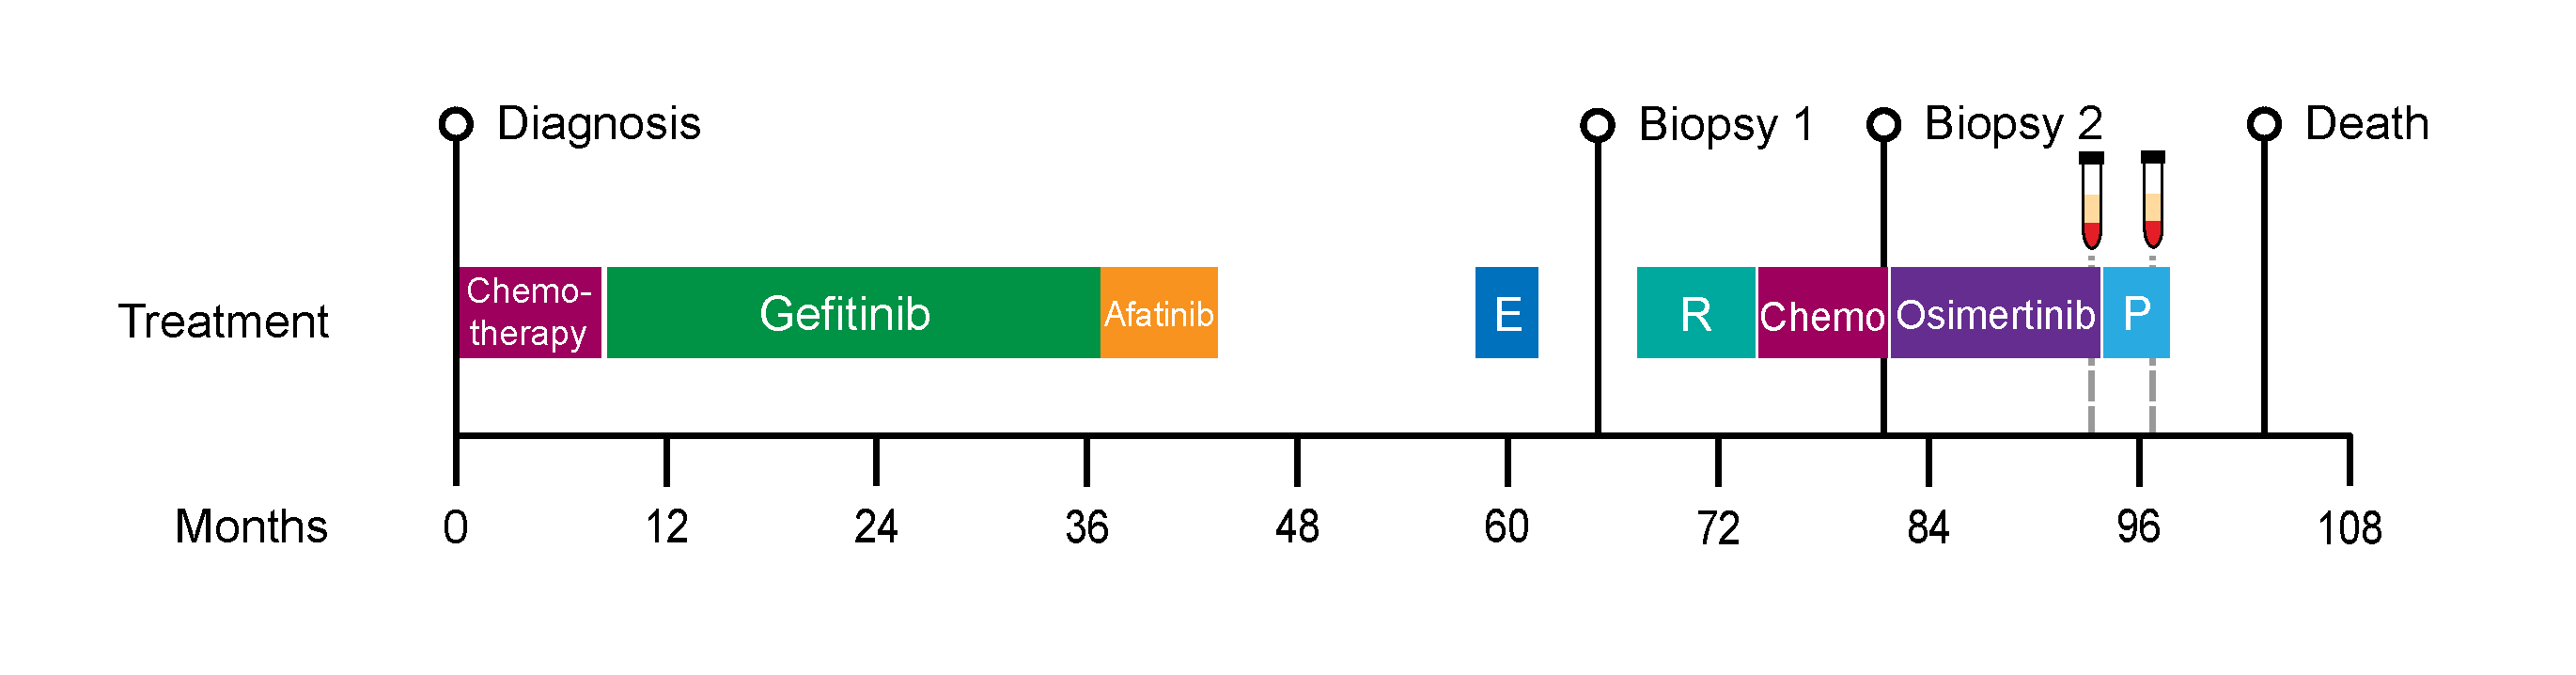
\includegraphics[width=.99\linewidth]{Figures/CASCADE/CA82/CA-K_timeline}
\caption[Timeline of patient CA-K from diagnosis until death]{Timeline of patient CA-K from diagnosis until death: Diagnostic biopsy detected EGFR~L858R positive lung adenocarcinoma;  Biopsy 1 after 66 months showed additional EGFR~T790M mutation; Biopsy 2 showed no additional variants; one blood sample was taken towards the end of Osimertinib treatment and one second one during PD-1 checkpoint blockade treatment. E: Erlotinib; R: Rociletinib; P: PD-1 inhibitor} \label{fig:ca82timeline}
\end{figure}




\begin{figure}[ht]
\centering
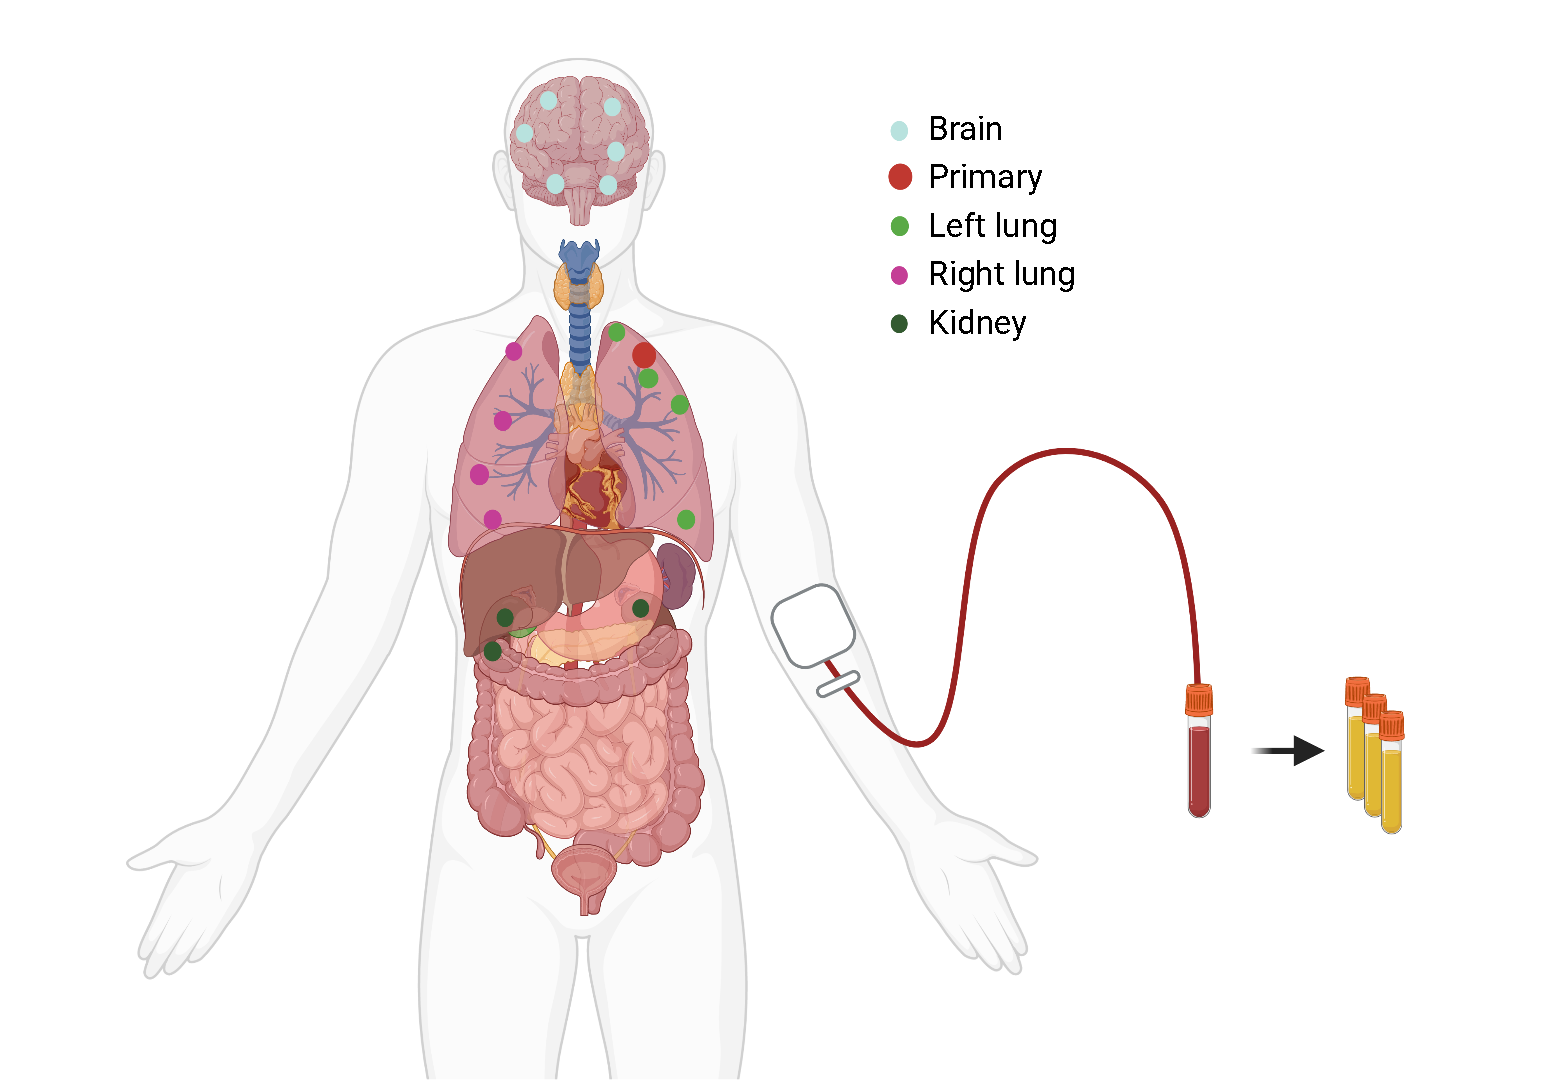
\includegraphics[width=.99\linewidth]{Figures/CASCADE/CA82/CA-K_schematic_CA82_organColours}
\caption[Schematic of analysed tumour lesions in patient CA-K]{Schematic of analysed tumour lesions in patient CA-K: Primary diagnostic sample shown in red; All 17 autopsy samples were coloured by organ they were collected from: Brain (6), left lung (4), right lung (4), kidney (3); Additionally to the post mortem blood sample, two serial blood samples were taken (\protect\autoref{fig:ca82timeline})} \label{fig:cas82schematic}
\end{figure}

\begin{table}[ht]
\caption[Autopsy samples sequenced for patient CA-K]{Autopsy samples sequenced for patient CA-K: Sample number is the internal sample collection during CASCADE autopsy, the organ of the sample, the fraction of tumour cell from H\& E stain and the pathology of the tumour sample. Dx: diagnostic sample}\label{tab:ca82wgsSamples}
\centering
\rowcolors{2}{gray!15}{white}
\begin{tabular}{|c|c|c|c|c|}
\toprule
\hline
 \rowcolor{gray!50}
\textbf{Sample number} & \textbf{Organ} & \textbf{H \& E} & \textbf{Type}\\
\hline
 Dx & left lung core & ? & \cellcolor{white} \\
 1 & right kidney & ? & \cellcolor{white} \\
 4 & right upper lung & ? & \cellcolor{white} \\
 5 & right lower lung & ? & \cellcolor{white} \\
 6 & right middle lung & ? & \cellcolor{white} \\
 8 & left lower lung & ? & \cellcolor{white} \\
 9 & left upper lung & ? & \cellcolor{white} \\
 13 & left brain & ? & \cellcolor{white}\multirow{-7}{*}{adenocarcinoma} \\
 \hline
\bottomrule
\end{tabular}
\end{table} 


\begin{table}[ht]
\caption[Copy number analysis results for patient CA-K]{Copy number analysis results for patient CA-K: results are taken from the best fit result of PURPLE; WG: whole genome}\label{tab:ca82cnv}
\centering
\rowcolors{2}{gray!15}{white}
\begin{tabular}{|c|c|c|c|c|}
\toprule
\hline
 \rowcolor{gray!50}
\textbf{Sample number} & \textbf{purity} & \textbf{ploidy} & \textbf{polyclonal \%} & \textbf{WG duplication}\\
\hline
 1 & \num{0.78} &	 \num{1.84} &	\num{7.62} & False	\\
 4 & \num{0.48} & \num{1.84} & \num{4.80} & False \\
 5 & \num{0.58} & \num{1.88} & \num{1.02} & False \\
 6 & \num{0.79} & \num{1.86} & \num{6.93} & False \\
 8 & \num{0.30} & \num{3.40} & \num{6.44} & True \\
 9 & \num{0.69} & \num{3.45} & \num{8.32} & True \\
 13 & \num{0.47} & \num{1.90} & \num{0.05} & False \\
 \hline
\bottomrule
\end{tabular}
\end{table} 


%we clear all floats before we go to the next patient
\cleardoublepage

%%%%%%%%%%%%%%%%%%%%%%%%%%%%%%%%%%%%%%%%%%%%%%%%%%%%%%%%%%%%%%%%%%%%%%%%%%%%%%%%%%%%%%%
%                               Patient CA86                                          %
%%%%%%%%%%%%%%%%%%%%%%%%%%%%%%%%%%%%%%%%%%%%%%%%%%%%%%%%%%%%%%%%%%%%%%%%%%%%%%%%%%%%%%%

\subsection{Patient CA-L}
\label{cascade-sec:CA86}

This 68 year old female ex-smoker presented with \textit{EGFR} mutant NSCLC, however after 12 months of the treatment with the EGFR inhibitor Erlotinib a transformation to small cell lung cancer (SCLC) was detected. While previously it was thought that the different subsets of lung cancers are distinct, more and more evidence is found showing neuroendocrine transformation as a resistance mechanism to targeted therapies not only in lung but also in prostate cancers \cite{Oser2015,Aggarwal2018}. The treatment was altered to chemotherapy and PD-1 inhibitors, however due to the loss of MHC-I antigen presentation of small cell lung cancer, the tumour failed to respond \cite{Burr2019} (\autoref{fig:ca86timeline}).

\begin{figure}[ht]
\centering
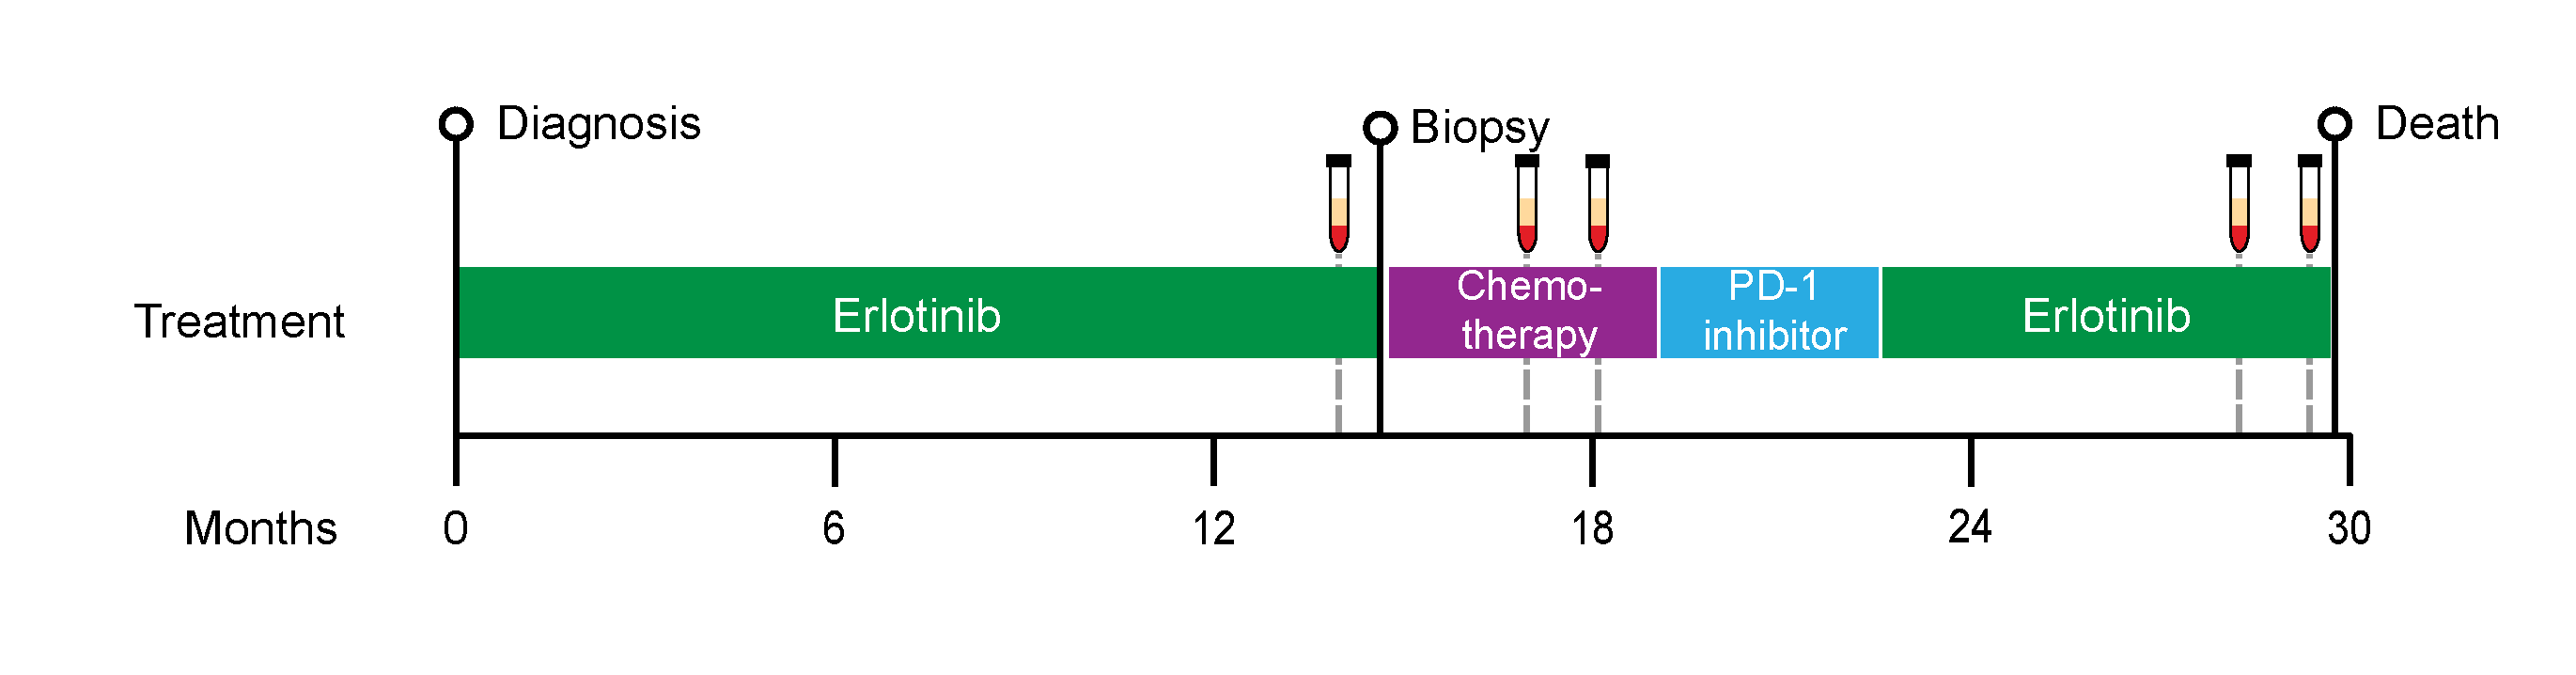
\includegraphics[width=.99\linewidth]{Figures/CASCADE/CA86/CA-L_timeline}
\caption[Timeline of patient CA-L from diagnosis until death]{Timeline of patient CA-L from diagnosis until death: Diagnostic biopsy detected EGFR exon 19 deletion positive lung adenocarcinoma;  Biopsy after 15 months Erlotinib treatment showed signs of small cell transformation; blood samples were taken at the end of the first Erlotinib treatment, during the chemotherapy treatment and  28 and 29 months after the initial diagnosis.} \label{fig:ca86timeline}
\end{figure}





\begin{figure}[ht]
\centering
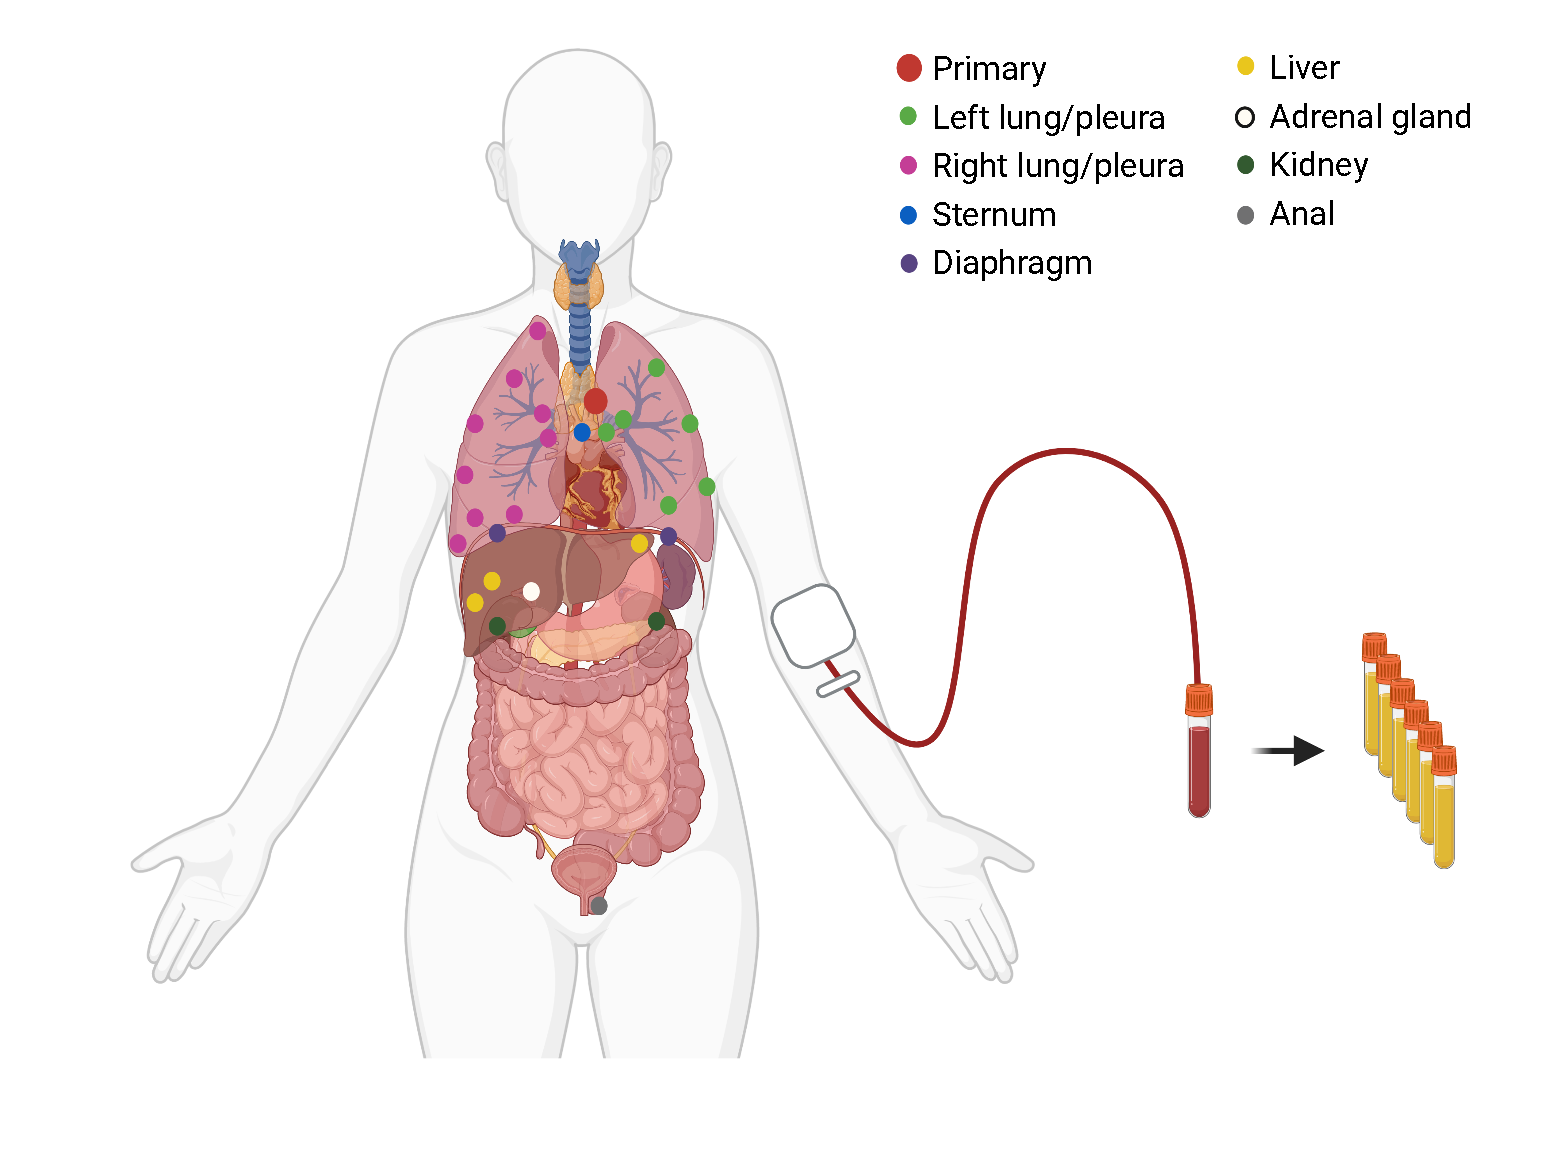
\includegraphics[width=.99\linewidth]{Figures/CASCADE/CA86/CA-L_schematic_CA86_organColours}
\caption[Schematic of analysed tumour lesions in patient CA-L]{Schematic of analysed tumour lesions in patient CA-L: Primary diagnostic sample shown in red; Samples are coloured by organ they were collected from: left lung (6), right lung (9), sternum (1), diaphragm (2), liver (3), adrenal gland (1) kidney (2), anal (1); Additionally to the post mortem blood sample, five serial blood samples were taken (\protect\autoref{fig:ca86timeline})} \label{fig:ca86schematic}
\end{figure}

\begin{table}[ht]
\caption[Autopsy samples sequenced for patient CA-L]{Autopsy samples sequenced for patient CA-L: Sample number is the internal sample collection during CASCADE autopsy, the organ of the sample, the fraction of tumour cell from H\& E stain and the pathology of the tumour sample. P.1/2: micro-dissected progression biopsy (80\% small cell, 20\% adeno)}\label{tab:ca86wesSamples}
\centering
\rowcolors{2}{gray!15}{white}
\begin{tabular}{|c|c|c|c|c|}
\toprule
\hline
 \rowcolor{gray!50}
\textbf{Sample number} & \textbf{Organ} & \textbf{H \& E} & \textbf{Type}\\
\hline
 P.1 & right lung core & \cellcolor{gray!15} & small cell \\
 P.2 & right lung core & \cellcolor{gray!15}\multirow{-2}{*}{>0.9} & adenocarcinoma \\
 8 & right upper lung & 0.9 & small cell \\
 17A & left lower lung & - & poorly differentiated adeno \\
 26 & right kidney & 1 & adenocarcinoma \\
 \hline
\bottomrule
\end{tabular}
\end{table} 

\todo[inline,color=red]{somatic variant calling analysis}

Copy number analysis with sequenza revealed a high prevalence of loss of heterozygosity in all samples (\Autoref{fig:ca86.p1circos,fig:ca86.p2circos,fig:ca86.8circos,fig:ca86.17Acircos,fig:ca86.26circos}), but both sample P.2 and 8 showed almost no copy number gains on chromosome 9 and 10 with 8 even extending through to 12. In general small cell transformed samples showed a higher level of copy number gain than the original adenocarcinoma. The difference in copy number in the two spatially intertwined types of cancers can only be attributed to the small cell transformation. Additionally to the increased overall ploidy of the small cell sample P.1 over P.2 (\autoref{tab:ca86cnv}), P.2 also lost chromosome X completely  (\autoref{fig:ca86.p1circos} vs. \autoref{fig:ca86.p2circos}). Interestingly, the small cell samples still have the same high amplification level of EGFR seen in the adenocarcinoma samples (min: 6 max: 13) suggesting the transformation was still in progress.

\begin{figure}[ht]
\centering
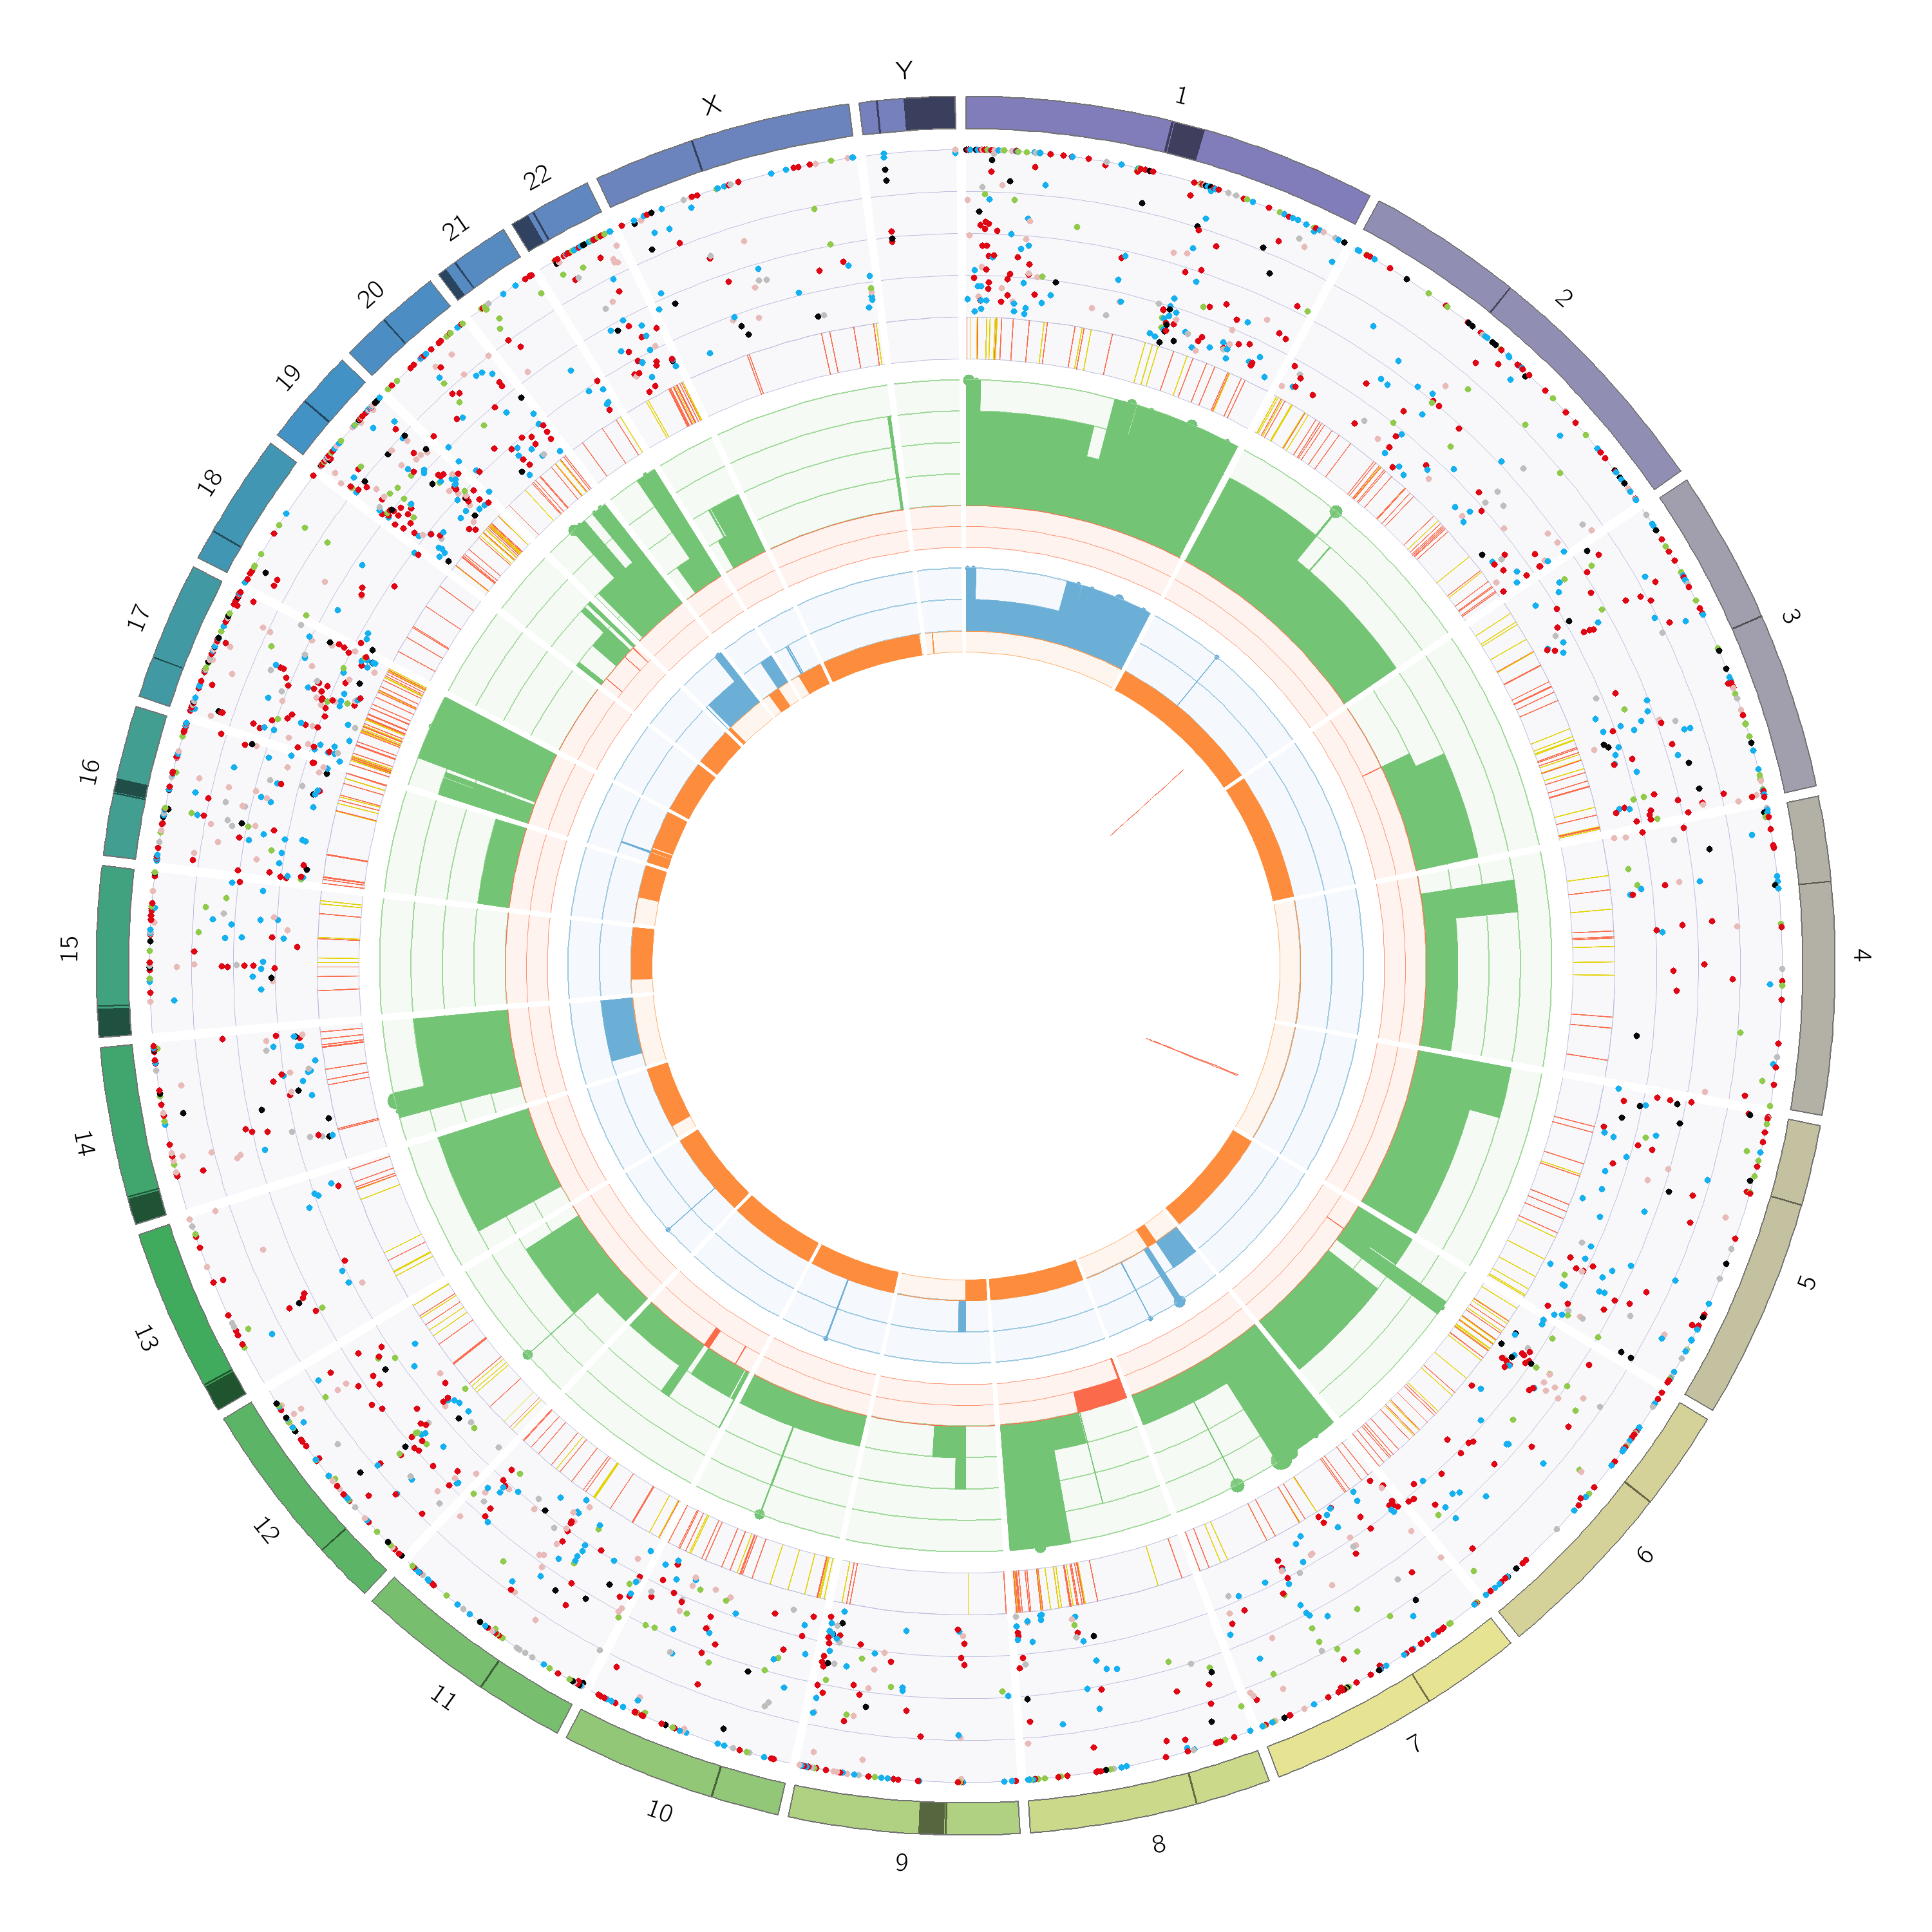
\includegraphics[width=.99\linewidth]{Figures/CASCADE/CA86/CA86-17B037524-1-S.circos.png}
\caption[Circos plot of patient CA-L sample P.1]{Circos plot of patient CA-L sample P.1: outer first ring shows the canonical chromosomes with gaps (centromere, heterochromatin,...) highlighted as darker areas; second ring visualises all somatic SNVs corrected for tumour purity and scaled from 0 to 1, the colour representing the base change of SNV like in \protect\textcite{Alexandrov2013}; vertical lines directly under the SNVs symbolise InDels, with yellow for insertions and red for deletions; the third ring shows the total copy number alterations, with green showing a copy number gain and red a loss, dots at the outer border show a copy number greater than four; the last ring shows the minor copy number, with blue depicting a gain and orange a loss, this ring allows the detection of copy number neutral changes, like loss of heterozygosity; the center shows all structural variants: translocations in blue, deletions in red, insertions in yellow, tandem duplications in green and inversions in black.} \label{fig:ca86.p1circos}
\end{figure}


\begin{figure}[ht]
\centering
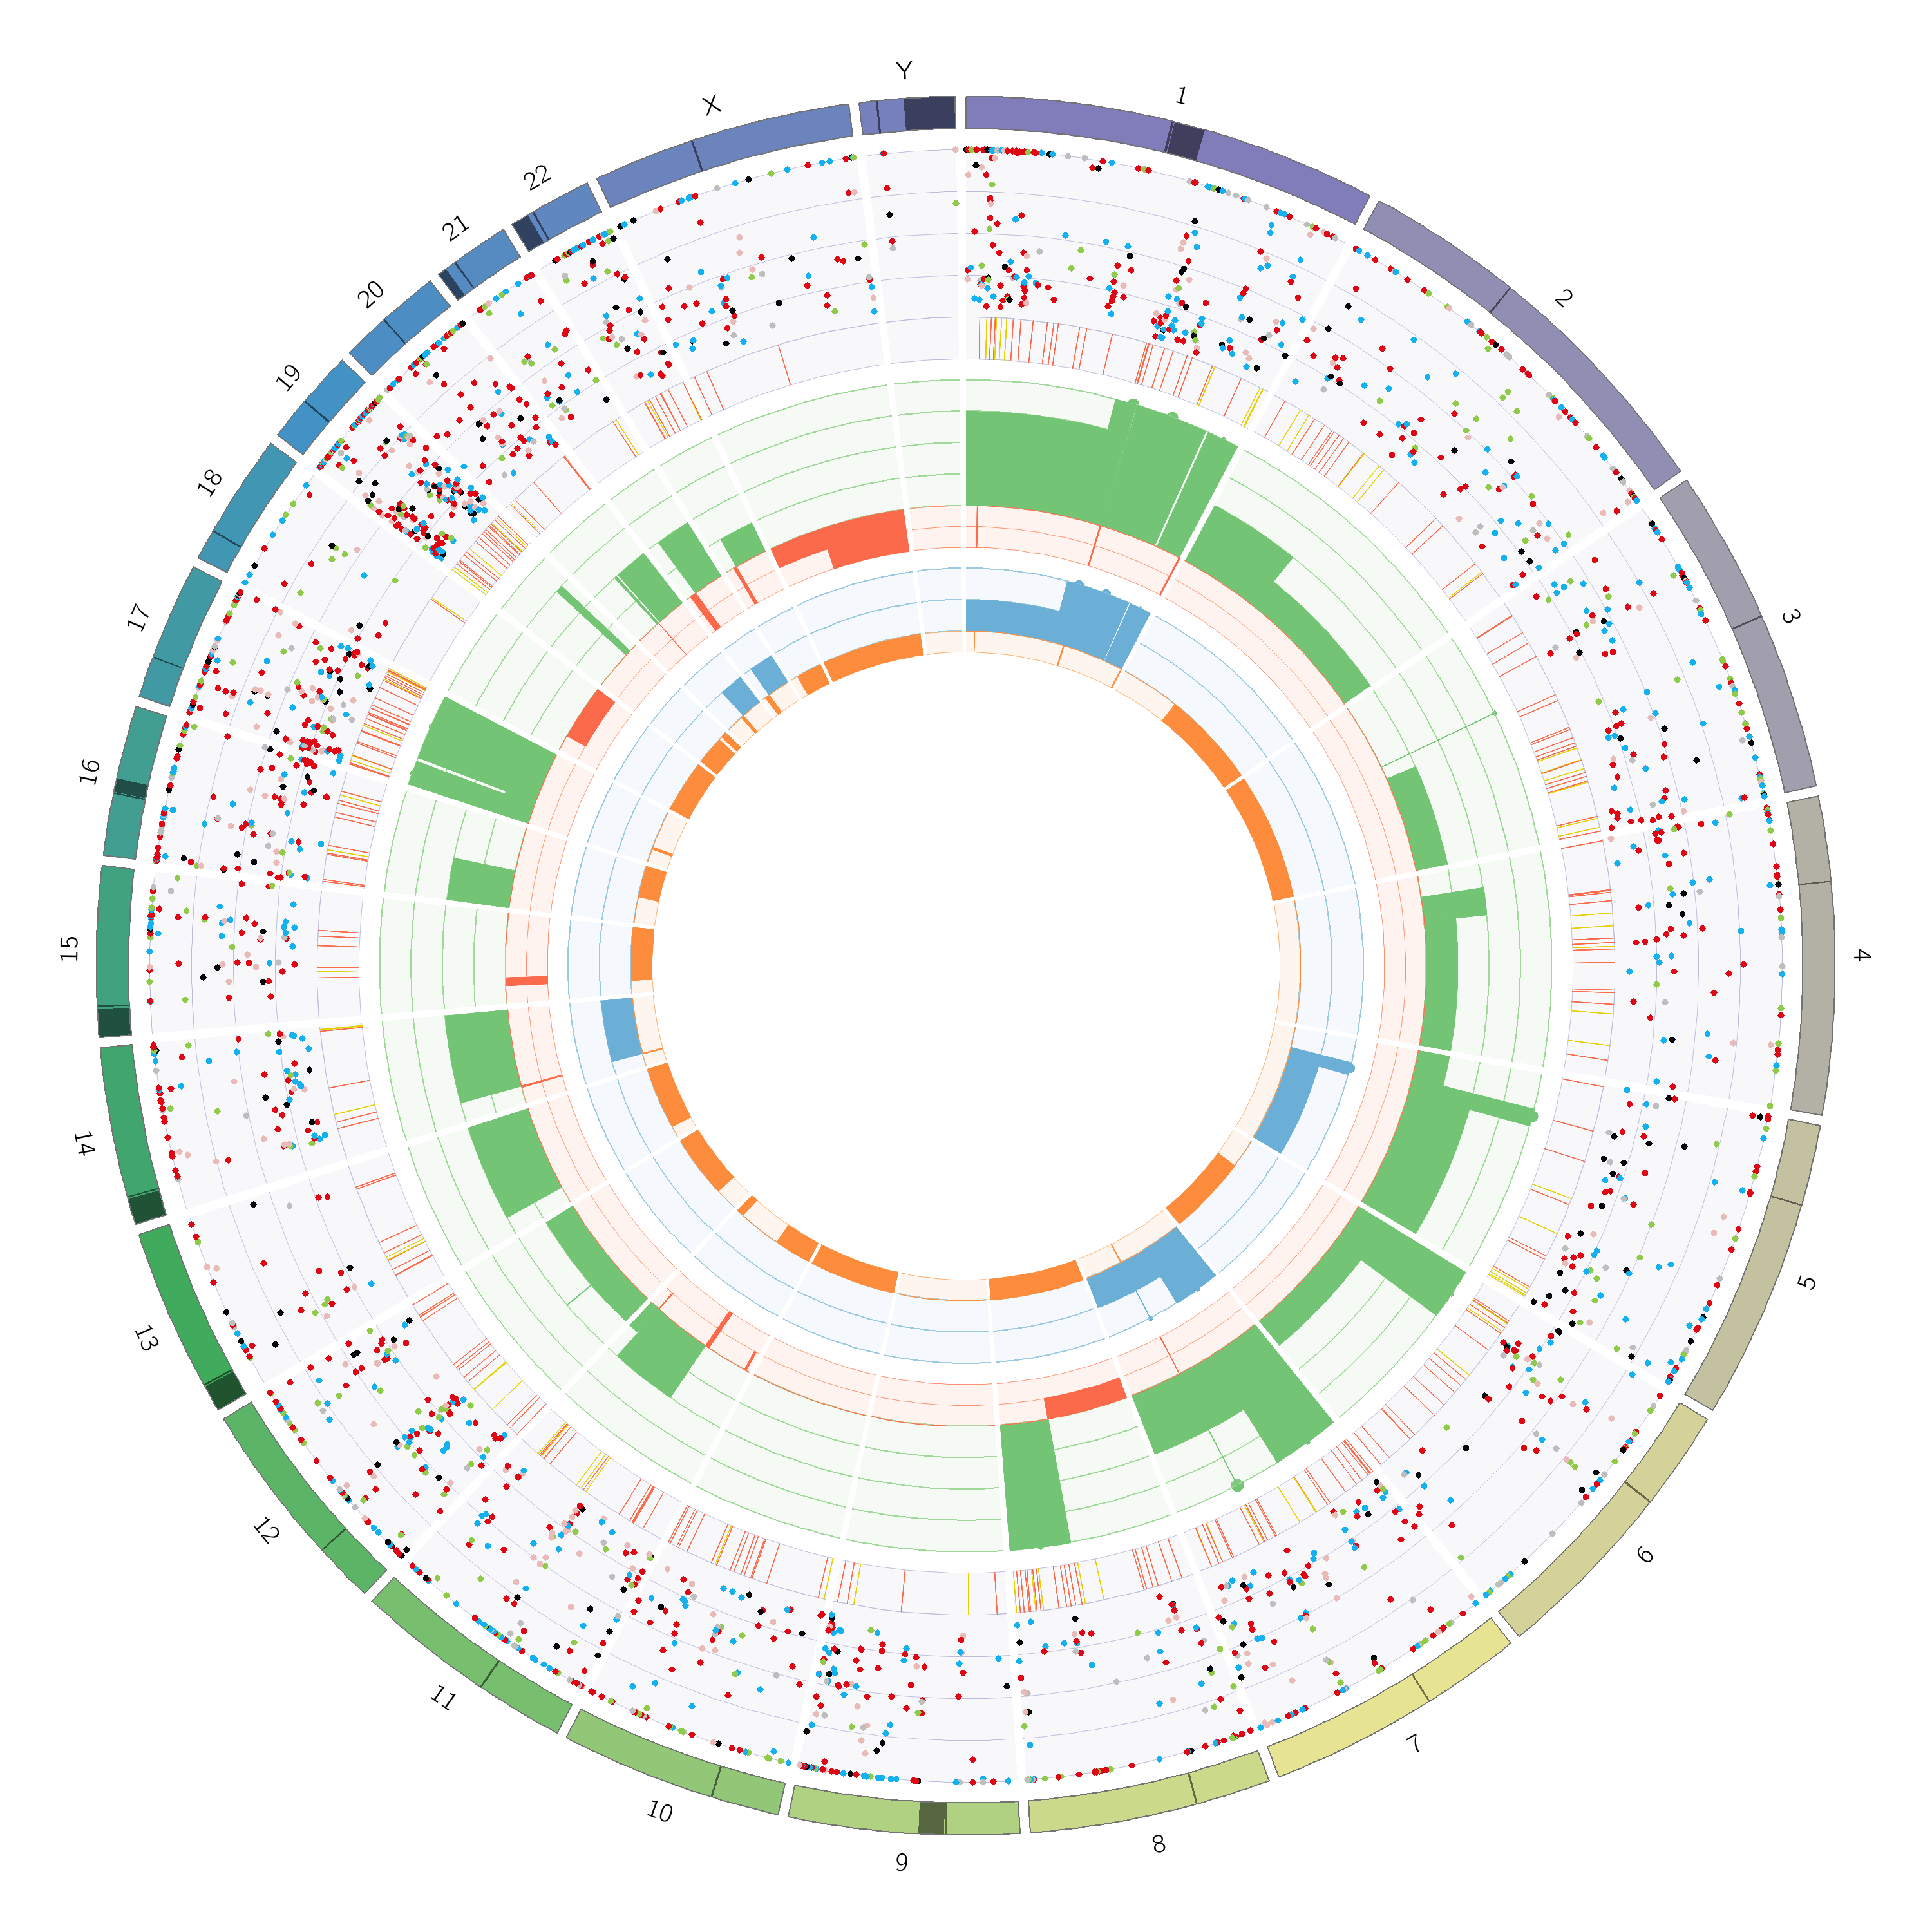
\includegraphics[width=.99\linewidth]{Figures/CASCADE/CA86/CA86-17B037524-1-A.circos.png}
\caption[Circos plot of patient CA-L sample P.2]{Circos plot of patient CA-L sample P.2: outer first ring shows the canonical chromosomes with gaps (centromere, heterochromatin,...) highlighted as darker areas; second ring visualises all somatic SNVs corrected for tumour purity and scaled from 0 to 1, the colour representing the base change of SNV like in \protect\textcite{Alexandrov2013}; vertical lines directly under the SNVs symbolise InDels, with yellow for insertions and red for deletions; the third ring shows the total copy number alterations, with green showing a copy number gain and red a loss, dots at the outer border show a copy number greater than four; the last ring shows the minor copy number, with blue depicting a gain and orange a loss, this ring allows the detection of copy number neutral changes, like loss of heterozygosity; the center shows all structural variants: translocations in blue, deletions in red, insertions in yellow, tandem duplications in green and inversions in black.} \label{fig:ca86.p2circos}
\end{figure}

\begin{table}[ht]
\caption[Copy number analysis results for patient CA-L]{Copy number analysis results for patient CA-L: results are taken from the best fit result of sequenza}\label{tab:ca86cnv}
\centering
\rowcolors{2}{gray!15}{white}
\begin{tabular}{|c|c|c|c|}
\toprule
\hline
 \rowcolor{gray!50}
\textbf{Sample number} & \textbf{purity} & \textbf{ploidy} & \textbf{WG duplication}\\
\hline
 P.1 & \num{0.86} &	 \num{3.3}  & True	\\
 P.2 & \num{0.27} & \num{2.1}  & False \\
 8 & \num{0.96} & \num{3.1}  & True \\
 17A & \num{0.18} & \num{4.2}  & True \\
 26 & \num{0.28} & \num{3.7} & True \\
 \hline
\bottomrule
\end{tabular}
\end{table} 

\todo[inline]{talk about the RNAseq data with RB1 loss in some areas}

%we clear all floats before we go to the next section
\cleardoublepage